\chapter{
Modeling Spatial Variation in Density
}
\markboth{Spatial Variation in Density}{}
\label{chapt.state-space}

\vspace{0.3cm}

Underlying every spatial capture-recapture models is a point process
that describes the number and distribution of animal activity
centers within the state-space ($\cal{S}$).
%, which is
%typically a two-dimensional polygon defining the study area.
A spatial point process is charcterized by %$\mathcal{S}$ and by
an intensity parameter defined at each location in $\mathcal{S}$; and
in the case of SCR models, this intensity parameter is population
density. If the intensity is constant, density is constant throughout
$\mathcal{S}$ and the point process is said to be homogeneous.
Thus far we have focused our attention on homogeneous %binomial
point processes whose realized values are the locations of the $N$
activity centers within the state-space. When a Poisson prior is
placed on $N$, we have a homogeneous Poisson point process, which
is referred to as a model of ``complete spatial randomness''.
%because the point process intensity is constant
%and the activity centers do not interact with one another.
A similar
model that we often use in conjunction with data augmentation and MCMC
is to place a binomial prior on $N$. This is also a model of spatial
randomness, and in this chapter we will compare and contrast the two.

The spatial randomness assumption is often viewed as restrictive
because ecological processes such as
territoriality and habitat selection can result in non-uniform
distributions of organisms. We have argued, however, that this
assumption is less restrictive than may be recognized because a
homogeneous point process actually allows for infinite
possible ``point patterns'', or realized configurations of activity
centers. Furthermore, given enough data,
the uniform prior will have very little influence on the estimated
locations of activity centers. Nonetheless, the homogeneous point
process model does not allow one to model population density using
covariates, which is an important objective in much ecological research.
For example, even when assuming a homogeneous point process model for
the activity centers, an estimated density surface may strongly
suggest that individuals are more abundant in one habitat than
another; however, such results do not provide the basis for formally testing
hypotheses about spatial variation in density, and they could not be
used to make predictions about habitat-specific abundance in other
regions. A more direct approach is to replace the homogeneous model
with an inhomogeneous model in which the point process intensity
is allowed to vary spatially.

In this chapter, we cover methods % we present a method
for fitting inhomogeneous Poisson and binomial
spatial point process models by treating the intensity parameter as a
function of covariates, in much the same way as is done in generalized linear
models. The covariates we consider differ
from those covered in previous chapters, which were typically
attributes of the animal (e.g. sex or age) or the trap (e.g. baited or
not) and were used to model movement or encounter
rate. In contrast, here we wish to model covariates that are defined
at all points in $\cal S$, which we will refer to as
state-space covariates or density covariates. These may
include continuous covariates such as elevation, or discrete
covariates such as habitat type. Such covariates are often formatted
as raster images with a prescribed resolution and extent.

Inhomogeneous Poisson point process models were discussed in the original
formulation of SCR models by \citet{efford:2004} and were described in
more detail by \citet{borchers_efford:2008}. We will show that an
inhomogeneous binomial point process is quite similar to the Poisson
model, but is more easily implemented in MCMC algortihms. To do so, we
will define the data augmentation parameter $\psi$ in terms of the point
process intensity function, and we will replace the uniform prior on the
activity centers with a prior that is also derived from the intensity
function. Development of this prior, which does not have a
standard form, is a central component of this chapter. First we
begin with a review of homogeneous point process models.


\section{Homogeneous point process revisited}

The homogeneous Poisson point process is \textit{the} model of ``complete
spatial randomness'' and is often used in ecology as a null model
to test for departures from randomness
\citep{cressie:1992, diggle:2003, illian_etal:2008}.
%Given its central role in spatial ecology, it is helpful to describe it briefly and
%compare it with the binomial model that we use in when conducting
%Bayesian analysis of SCR models.
As with all homogeneous point process models, the Poisson model
asserts that the realized points do not interact with each other in
any way---for example, they neither attract nor repel one another.
This model also posits that the number of points in $\mathcal{S}$ is
Poisson distributed: $N \sim \text{Poisson}(\mu|\mathcal{S}|)$ where $\mu>0$ is
the intensity parameter and $|\mathcal{S}|$ is the area of the
state-space. The intensity parameter $\mu$
is the density of points, and thus multiplying the intensity by the area
of some region yields the expected number of points in that region.

Unlike the Poisson point process, the
binomial point process assumes that $N$ is fixed, not random.
%In other words, the binomial point process conditions on $N$,
as is illustrated by this simple \R~code that generates realizations
from Poisson and binomial point processes in the unit square
($\mathcal{S} = [0,1]\times[0,1]$):

\begin{samepage}
\begin{verbatim}
Area <- 1                          # Area of unit square
muP <- 4                           # intensity
nP <- rpois(1, muP*Area)           # number of points: random
PPP <- cbind(runif(nP), runif(nP)) # Poisson point pattern

nB <- 4                            # number of points: fixed
muB <- nB/Area                     # intensity
BPP <- cbind(runif(nB), runif(nB)) # binomial point pattern
\end{verbatim}
\end{samepage}

{\flushleft Both of these models are homogeneous because the intensity parameter
is constant ($\mu=4$ in both cases) and the $N$ points do not interact
with each other. This results from the fact that the locations of the
points follow a uniform distribution on the plane. The key distinction
is that $N$ is random in the former and fixed in the latter.}

Another difference between the Poisson and binomial models is that if the
state-space is divided into $K$ disjunct regions, the number of points in each
region $n(B_k): k=1,\dots,K$; are independent and identically
distributed (i.i.d.) under the Poisson model but not under the
binomial model. In the Poisson case,
the counts are simply distributed as $n(B_k) \sim
\text{Poisson}(\mu|B_k|)$, where $|B_k|$ is the area of the region
$B_k$. For the binomial case, $n(B_k) \sim
\text{Binomial}(N, \pi(B_k))$ where $\pi(B_k)$ is the proportion of
the state-space in $B_k$; however, these counts are not
i.i.d. because the number of points in one region is informative
about the number of points in another region. For example, if
$N=10$, which would be known for a binomial point process, and if we
know that there are 7 points outside the region $B_1$,
then we can say with certainty that $B_1 = 10 - 7 = 3$.

Fig.~\ref{state-space.fig.homo} is meant to further illustrate the characteristics
of the binomial model. The left panel shows a point pattern
realized from a
homogeneous binomial point process with $N=50$. The right panel shows
the same realization, except that the state-space has been discretized
into 25 equally-sized disjunct regions, or pixels, and the counts in each pixel
are shown. Since the pixels are the same
size, $\pi(B_k) = 1/25$, the expected number of point in each
pixel is 2: $\mathbb{E}(n(B_k)) = N\pi(B_k) = 50/25$, which
happens to be the empirical mean in this instance. However, as
previously stated, these counts are not
independent realizations from a binomial distribution since $\sum_k
n(B_k) = N$. Rather, the model for the entire vector is multinomial:
$\{n(B_1), n(B_2), \dots, n(B_k)\} \sim \mbox{Multinomial}(N, \{p(B_1), p(B_2), \dots,
p(B_K) \})$ \citep{illian_etal:2008}. If you need a refresher on the
multinomial distribution, refer to Sec.~\ref{modeling.sec.multinom}, and
consider the following \R~code, which generates counts such as those
seen in Fig.~\ref{state-space.fig.homo}:
\begin{verbatim}
n.Bk <- rmultinom(1, size=50, prob=rep(1/25, 25))
matrix(n.Bk, 5, 5)
\end{verbatim}

\begin{figure}%[ht!]
\centering
%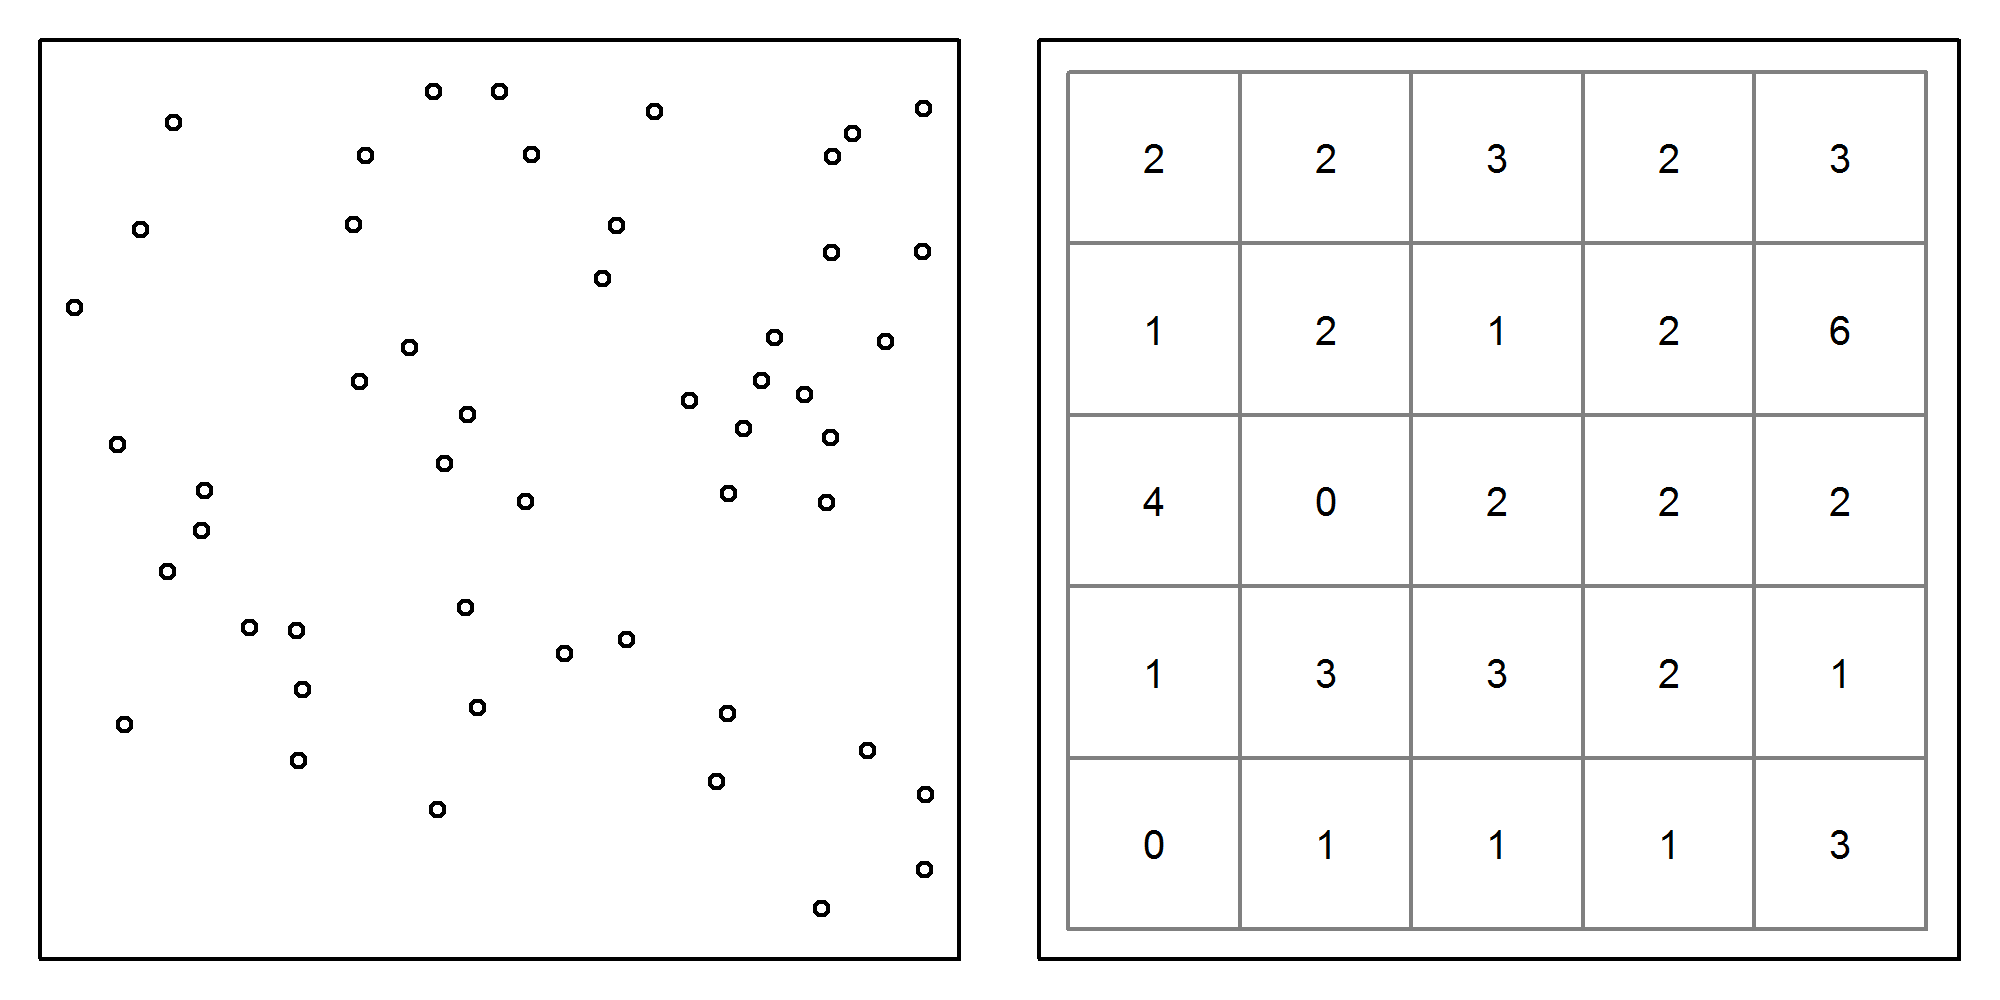
\includegraphics[width=5in,height=2.5in]{Ch11/figs/homoPlots}
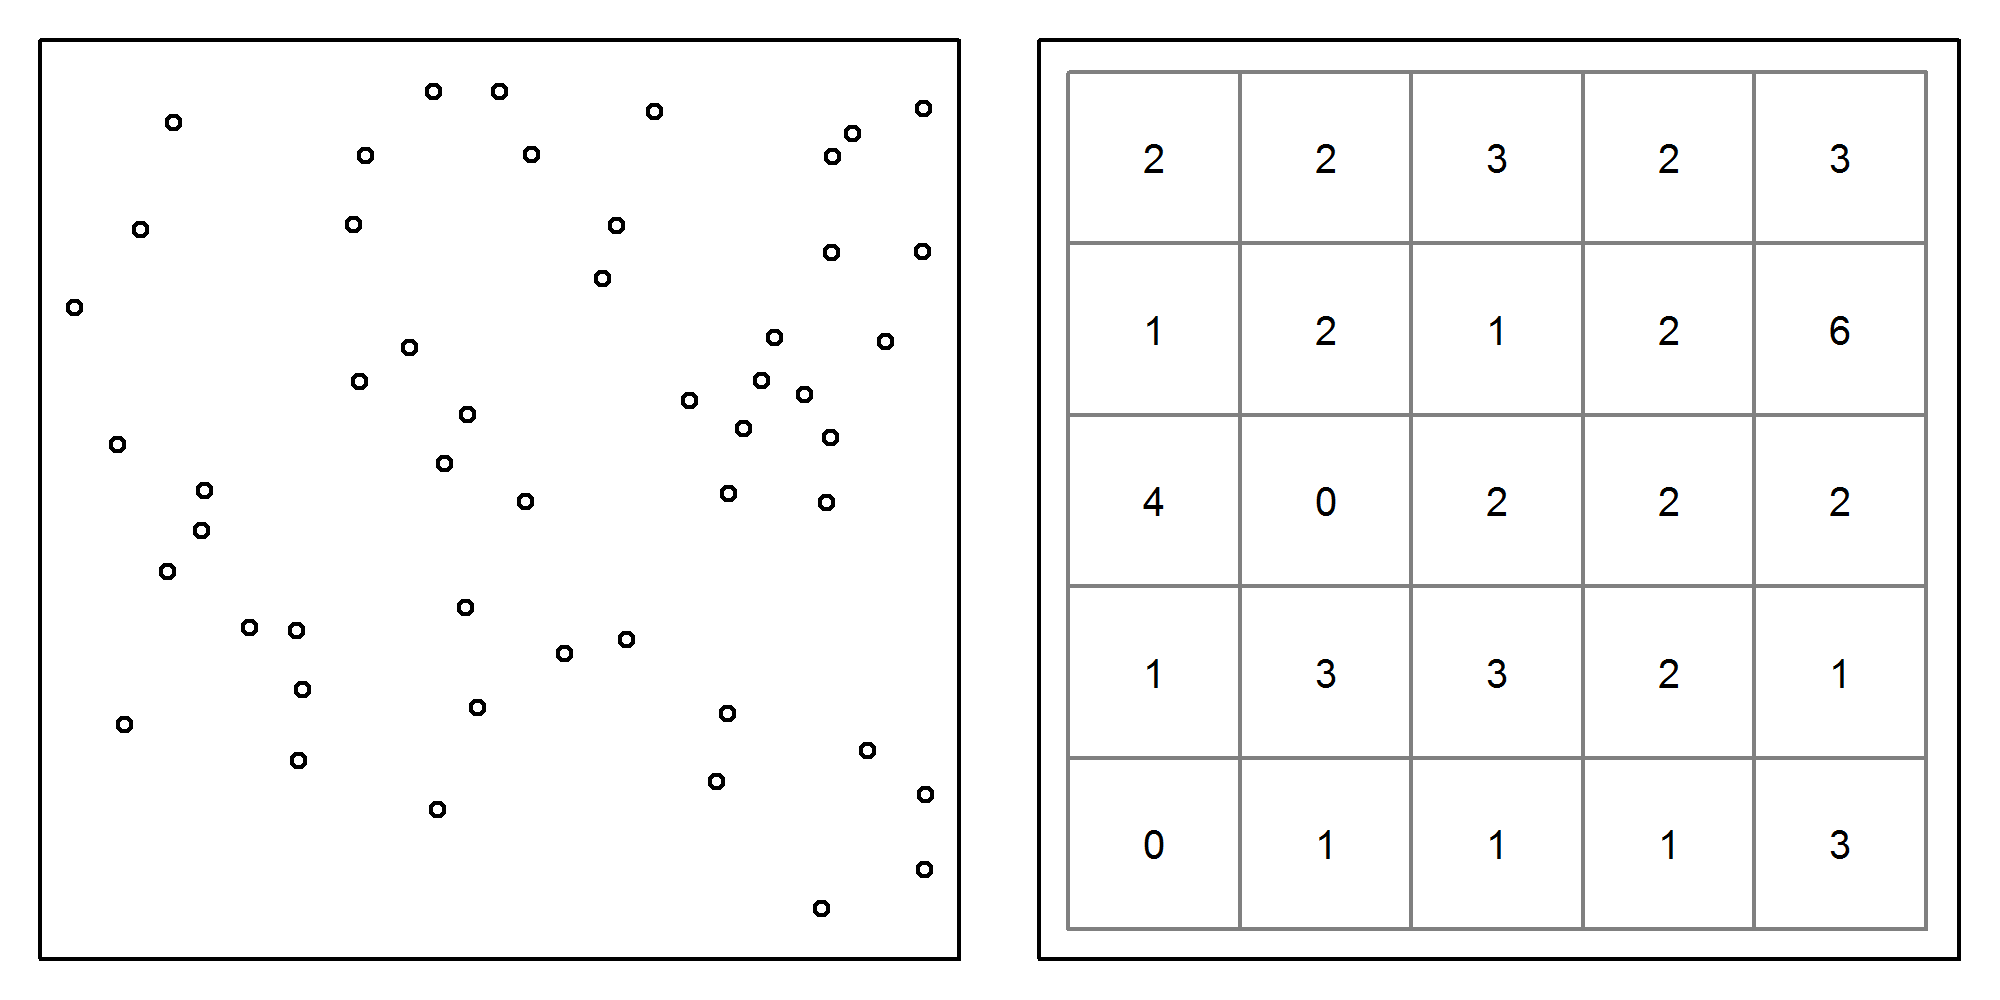
\includegraphics[width=\textwidth]{Ch11/figs/homoPlots}
\label{state-space.fig.homo}
\caption{Homogeneous binomial point process with $N$=50 points
  represented in continuous and discrete space.}
\end{figure}

The dependence among counts has virtually
no practical consequence when the number of pixels is large. For
example, if there are 100 pixels, the number of points in one pixels
carries very little information about the expected number of points in another
pixel. However, if there are only 2 pixels, then clearly the number of
points in one pixel allows one to determine how many points will occur in the
remaining pixel.

The discrete representation of space shown in
Fig.~\ref{state-space.fig.homo} is not only helpful for understanding
the properties of a point process, it is also of practical importance
when fitting SCR models because spatial covariates are almost always
represented in as rasters. In such cases, the definition of the prior for
the point locations can be changed from the probability that a point
occurs at some location in space to the probability that it occurs in
some pixel of the raster. As we will explain in
Sec.~\ref{modeling.sec.discrete}, this typically involves changing the
prior from a uniform distribution to a multinomial or categorical
distribution.

Up to this point in this chapter we have sketched out the basic characteristics
of homogeneous Poisson and binomial point process models. Now we need
to speak more specifically about their relevance to SCR models before we move on
to the inhomogeneous models. %Much of this has already been in previous
%chapters, but we feel it is important enough to review here.
In a SCR model with a homogeneous point process, the intensity
parameter $\mu$ is interpretted as population density, and $N$ is
interpretted as population size\footnote{Strictly speaking, $N$ is the
  number of activity centers in $\mathcal{S}$}. These interpretations
are true regardless of whether we consider the
Poisson model or the binomial model, but since $N$ is always unknown, one
might wonder why we are discussing the binomial model at all. %Indeed,
%the binomial model was not mentioned by \citet{efford:2004} or
%\citet{borchers_efford:2008}. Instead, they focused exclusively on the
%Poisson model and estimation of $\mu$, with $N$ being regarded as a
%derived parameter.

In our work, we typically adopt the binomial model simply
because it is easy to implement using MCMC and data
augmentation. And while $N$ is truly unknown, we use an upper bound $M$
which is fixed. Thus, the standard point process we use Bayesian
analyses can be
regarded in two ways. First, it is a binomial point process with $M$
points. Second, in terms of $N$, it is a thinned binomial point
process, where $\psi$ is the thinning parameter.
\hl{XXXX Is this thinned point process also binomial, even though N is
  no longer fixed? XXXX}.
With this in mind,
the only real difference between the Poisson and binomial models, as
implemented in SCR contexts, is that in the former, we have
$N \sim \text{Poisson}(\mu|\mathcal{S})$, and in the latter we have
$N \sim \text{Binomial}(M, \psi)$. In other words, we just have a
different prior on $N$, and when using MCMC, the binomial prior is
much more convienient becuase it fixes the size of the parameter space
and makes it easy to extend the model in each of the ways discussed in
this book. It is also worth remembering that the Poisson
distribution is the limit of the binomial distribution when $M$ is
very high and $\psi$ is very low (Chapt.~\ref{chapt.modeling}), and
thus the two models are much more similar than may appear.

You might have noticed that the intensity parameter $\mu$ was not shown for the
binomial prior $N \sim \text{Binomial}(M, \psi)$. Instead, we see the
data augmentation parameter $\psi$, which has been used throughout
this book, but without much mention of the point process
intensity. What then is the relationship between $\psi$ and $\mu$?
As first discussed in Chapt.\ref{chapt.scr0}, under data augmentation,
the expected value of $N$ is $\mathbb{E}[N] = M\psi$. But, from this
chapter, we also know that the
expected value of $N$ can be written in terms of $\mu$ as
$\mathbb{E}[N] = \mu|\mathcal{S}|$. Therefore,
$\psi = \mu|\mathcal{S}| / M$ and hence we can directly estimate $\mu$
rather than $\psi$ if we so desire---and we will so desire in the next
section where the objective is to model $\mu$ as a function of
spatially-referenced covariates. First, as an exercise, execute the
following \R~commands to familiarize yourself with some of the
concepts we just covered:
\begin{small}
\begin{verbatim}
Area <- 1                  # Area of state-space
M <- 100                   # Data augmentation size
mu <- 10                   # Intensity (points per area)
psi <- (mu*Area)/M         # Data augmentation parameter (thinning rate)
N <- rbinom(M, 1, psi)     # Realized value of N under binomial prior
cbind(runif(N), runif(N))  # Point pattern from thinned binomial model
\end{verbatim}
\end{small}
%This code illustrates the fact that $\psi$ can be expressed as a
%function of the point process intensity $\mu$. Thus each and every
%MCMC algorithm used in this book could have been parameterized in
%terms of $\mu$ rather than $\psi$. However, you might have noticed
%that the above code does not include the indicator variables

\begin{comment}
  We conclude this section by pointing out
  Table\ref{state-space.tab.pvb}, which highlights the differences of
  the homogeneous Poisson and binomial point process models as they
  relate to SCR. % XXXX Need to fill in this table XXXX

\begin{table}
  \centering
  \caption{Characteristics of homogeneous point
    processes. Table~\ref{state-space.tab.hetero} describes the
    inhomogeneous models.}
  \begin{tabular}{lccc}
    \hline
    & Prior & $\mathbb{E}[N]$    & $\mu$   \\
    \hline
    Poisson  & $N \sim \text{Poisson}(\mu|\mathcal{S}|)$   &  &  \\
    Binomial & $N \sim \text{Binomial}(M, $   & $M\psi = $   &  &  \\
    \hline
  \end{tabular}
  \label{state-space.tab.homo}
\end{table}
\end{comment}


\section{Inhomogeneous point processes}

The principal difference between homogeneous and inhomogeneous point
processes is that the intensity parameter $\mu$ is allowed to vary spatially
in the inhomogeneous model. Thus, rather than $\mu$ being a fixed constant,
it is now a function defined at each point $\mathbf{s} \in
\mathcal{S}$. A vast number of options exist for modeling spatial
variation in the intensity of a point process
\citep{cox:1955,stoyan_penttinen:2000,illian_etal:2008}, but here we
focus on modeling $\mu$ as a function of
spatially-referenced covariates and a vector of regression
coefficients $\bm \beta$; a function we will denote $\mu(\mathbf{s},
\bm{\beta})$. To be clear, $\mu(\mathbf{s}, \bm{\beta})$, is a
function that returns the expected density of activity centers at
location $\bf s$, given the covariate values at $\bf s$.  Since the
intensity must be positive, and because the natural logarithm is the
canonical link function of the Poisson generalized linear model
\citep{mccullagh_nelder:1989}, it is natural to consider the following model:
\begin{equation}
  \log(\mu(\mathbf{s}, {\bm \beta})) = \beta_0 + \sum_{v=1}^V \beta_v z_v(\mathbf{s})%, \quad  \mathbf{s} \in \cal{S}
  \label{state-space.eq.loglin}
\end{equation}
which says that there are $V$ covariates and $\beta_v$ is the
regression coefficient for covariate $z_v(\mathbf{s})$. This
covariate, $z_v(\mathbf{s})$, could be any variable defined at all points
in the state-space, such as habitat type or elevation.
Eq.~\ref{state-space.eq.loglin} should look familiar because it is the
standard linear predictor used in Poisson regression. As with other
GLMs, one could consider alternative link functions.

Recall from the previous section that for a homogeneous point process,
the expected number of points in the state-space was simply the
intensity parameter multiplied by area: $\mathbb{E}[N] =
\mu|\mathcal{S}|$. But now that we are regarding the intensity as a
function, rather than a scalar, this equation is not very useful. So
what is $\mathbb{E}[N]$ for an inhomogeneous point process?
%And why do
%we care? Well, hopefully you remember that the reason we need a
%the reason we care is that we want a model that
Contemplating a discrete state-space is useful for figuring this
out. Imagine that the state-space is represented as a raster with many
tiny pixels. In this case, we will associate
$\bf s$ with pixel ID, i.e. $\bf s$ just references some pixel that
has $V$ covariates values associated with it. The expected number of
individuals in this pixel, say $\mathbb{E}[n(\mathbf{s})]$, can intuitively be
found by evaluating the intensity function
(Eq.~\ref{state-space.eq.loglin}) and multiplying it by the area of
the pixel. In other words, we compute the exptected number of
individuals in a pixel by multiplying the expected value of density
for that pixle by the area of the pixel. If we do this for each pixel in the state-space, then
summing up these values gives us what we are after, the expected value
of $N$. Specifically,
$\mathbb{E}[N] = \sum_{\mathbf{s} \in \mathcal{S}} \mathbb{E}[n(\mathbf{s})]$.
As the area of the pixels approaches zero, such that we move from discrete
space back to continuous space, the summation must be replaced
with an integration of the form:
\begin{equation}
\mathbb{E}[N] = \int_{\mathcal{S}} \mu(\mathbf{s}, {\bm \beta}) \mathrm{d}\mathbf{s}
\label{state-space.eq.EN}
\end{equation}
This is an important equation because, once the $\bm \beta$ parameters
have been estimated, it can be used to make predictions
about abundance for any spatial region.

We have now described an approach for modeling the point process
intensity, yet in order to define the likelihood or to develop an MCMC
algorithm for the inhomogeneous model, we need to specify the prior
distribution for the activity centers. Recall that under the
homogeneous point process, the prior was
$\mathbf{s}_i \sim \text{Uniform}(\mathcal{S})$, for $i=1,\dots,N$, or
equivalently:
\begin{equation}
  \label{state-space.eq.uprior}
  [\mathbf{s}_i] = 1/|\mathcal{S}|
\end{equation}
where once again $|\mathcal{S}|$ denotes the area of the
state-space. This simply indicates that an activity center is equally
likely to occur at any location in the state-space.
However, if animals exhibit habitat selection or simply
occur in one region more often than another, it would be preferable to
replace this prior with one describing the spatial variation in
density. Clearly this prior should be determined in some way by the
spatially-varying intensity function $\mu(s, \bm{\beta})$.
The key to determining this prior is to recall that
the integral of a probability density function (pdf) must be unity,
and we can always convert any function into a pdf by dividing it by a
normalzing constant. In this case, the normalizing constant is the integral
of $\mu(s, \bm{\beta})$ evaluated over the entire state-space.
The probability density function of the new prior is therefore:
\begin{equation}
[\mathbf{s}_i | \bm{\beta}] = \frac{\mu(\mathbf{s}_i, \bm{\beta})}{\int_{\mathcal{S}} \mu(\mathbf{s}, \bm{\beta})\, \mathrm{d}\mathbf{s}}
\label{state-space.eq.pdf.hetero}
\end{equation}
Substituting the uniform prior with this new distribution
allows us to fit inhomogeneous binomial point process
models to spatial capture-recapture data.
%We can also use this
%distribution to obtain the expected number of individuals in any given
%region $B \in \mathcal{S}$. Specifically, the proportion of $N$ expected to occur in
%$B$ is $\pi(B) = \int_B [\mathbf{s} | \bm{\beta}]\, \mathrm{d}x$. These are
%also the conditional-on-$N$ multinomial cell probabilities if the regions are
%disjoint and compose the entire state-space. We provide an example in
%the next section, and in Fig.\ref{state-space.fig.hetero}.

As a practical matter, note that the integral in the
denominator of Eq.~\ref{state-space.eq.pdf.hetero} is evaluated over
space, and since we always regard space as two-dimensional (the
state-space is planar), this is a two-dimensional integral that can
be approximated using the methods discussed in
Chapter~\ref{chapt.poisson-mn}, which include
Monte Carlo integration and Gaussian quadrature. Alternatively, if
our state-space covariates are in raster format, i. e. they are
in discrete space, the integral can be replaced with a sum over
all the pixels in the raster,
\begin{equation}
[\mathbf{s}_i | \bm{\beta}] = \frac{\mu(\mathbf{s}_i, \bm{\beta})}{\sum_{\mathbf{s} \in \mathcal{S}} \mu(\mathbf{s}, \bm{\beta})}
\label{state-space.eq.pdf.hetero.d}
\end{equation}
where $\bf s$ is now defined as ``pixel ID'' rather than a point in space.

Although the discrete space approach is standard practice, it is
technically unjustified because covariate values must be known for all
points in space. This same problem is present anytime that we have a
sample of the spatial covariates, rather than a function defining
their value for all points in space. In such cases, it may be necessary to
interpolate the values of the covariates for points in space where
they were not measured. One option would be to use a Kriging
interpolator, as demonstrated by \citet{rathbun:1996}. Another option
is to sample the spatial covariates using probabalistic sampling
methods, which allow for design-based estimators of their values for
the entire study area \citep{rathbun_etal:2007}. Either option could
be implemented within maximum likelihood or MCMC estimation methods; however, even though such
approaches are technically necessary, we do not demonstrate them here
because it seems likely that they will be inconsequential in most
cases where the raster data are of high resolution, such that the loss
of information is negligible when going from continuous space to
discrete space. Furthermore, the validity of this assertion, and the
level of resolution required to adequately approximate continuous
space can often be assessed by checking the consistency of the
parameter estimates among varying levels of resolution, as was
demonstrated in Chapt.~\ref{chapt-scr0}.

We now have all the tools needed to fit inhomogeneous point process
models. Likelihood-based inference for inhomogeneous Poisson point
process models was described by \citet{borchers_efford:2008} and
reviewed in Chapt.~\ref{chapt.mle}. Another example is demonstrated in
the next section, but first we focus on the binomial
model that we favor when conducting Bayesian inference. In the
previous section we noted that the data augmenation parameter $\psi$
can be expressed in terms of the intensity parameter $\mu$. The same
is true for inhomogeneous models. Specifically, rather than
$\mathbb{E}[N] = \psi M$ as before, we use expected value of $N$ shown
in Eq.~\ref{state-space.eq.EN} which results in
\begin{equation}
\psi = \frac{\int_{\mathcal{S}} \mu(\mathbf{s},
  \bm{\beta}) \, \mathrm{d}\mathbf{s}}{M}
\label{state-space.eq.psimu}
\end{equation}
As before, the data augmentation limit $M$ must be high enough so that
it is greater than the numerator---i.e. the expected value
of $N$ must be less than $M$.

If we refer to the distribution $[\mathbf{s}_i | \bm{\beta}]$ as
``IPP'', we can write a hierarchical description of a SCR model with a
Binomial encounter process and a half-normal detection function as
\begin{gather*}
w_i \sim \mbox{Bernoulli}(\psi) \\
{\bf s_i} \sim \mbox{IPP}(\mu(s,\beta)) \\
p_{ij} = p_0 \exp(-\|{\bf s_i} - {\bf x_{j}}\|^2/(2\sigma^2)) \\
y_{ij} \sim \mbox{Binomial}(K, p_{ij} w_i)
\end{gather*}
The new prior for $\mathbf{s}_i$ and Eq.~\ref{state-space.eq.psimu}
%use of $\mbox{IPP}(\mu(s, \beta))$ instead of
%$\mbox{Uniform}(\cal{S})$ is the
are the key differences between homogeneous an inhomogeneous
models. %, and the %two are equivalent when $\bm{\beta}=0$.

\begin{comment}
The IPP for the activity centers
results in another IPP for the observation process, $\lambda(s)$, the
expected number of captures for a trap
at point. As was true for the homogeneous model, this
intensity function is a product of the point process intensity
and the encounter rate function, $\lambda(s) = \mu(s, {\bm \beta})
\lambda_{ij}$.
\end{comment}

In the next sections we walk through a few examples, building up from
the simplest case where we actually observe the activity centers as
though they were data. In the second example, we fit our new model to simulated
data in which density is a function of a single continuous
covariate. To build upon the developments in the previous chapter, we
further consider the plausible case where a state-space covariate is also a
covariate of ecological distance. A small simulation study indicates
that both effects can be estimated. A fourth example shows an analysis in discrete space using
both \secr~\citep{efford:2011} and \jags~\citep{plummer:2003}. In the
fifth and final example, we model the intensity of
activity centers for a real dataset collected on jaguars
(\emph{Panthera onca}) in Argentina.

\section{Observed Point Processes}

In SCR models, the points (activity centers) are not directly
observed, but in other contexts they are. Examples include the
locations of disease outbreaks, the locations of trees in a forest, or
the locations of radio-tracked animals. In such cases, it is
straightforward to fit inhomogeneous point process models and estimate the
%Indeed Eq.~\ref{eq.pdf.ipp}
%has been used extensively in the radio-telemetry literature to model
%so-called ``resource selection functions''
%\citep{manly_etal:2002,lele_keim:2006}. When the point locations are
%directly observed, estimating
the parameters $\bm \beta$ from Eq.~\ref{state-space.eq.loglin}, as we
will do in the following example. % is
%straight-forward as demonstrated in the following example.
%This example also illustrates the fundamental process that we will
%later embed in our MCMC algorithm used to fit SCR models that include
%an inhomogeneous point process.

Suppose we knew the locations of $N$ animal activity
centers, perhaps as the result of an extensive telemetry study. %To
%estimate the intensity surface $\mu(\mathbf{s}, \bm{\beta})$ underlying these
%points, we need to derive the likelihood for the data under this
%model.
If we assume $N$ is Poisson distributed and the points are
mutually independent of one another, we can fit the
inhomogeneous Poisson point process model whose likelihood is
the product of $N$ densities given by
Eq.~\ref{state-space.eq.pdf.hetero} \citep[pg. 104]{diggle:2003}. The
log-likelihood is thus:
\[
\ell({\bm \beta} | \{{\bf s}_i\}) = \sum_{i=1}^N
\log(\mu(\mathbf{s}_i, \bm{\beta})) - \int_{\mathcal{S}} \mu(\mathbf{s}, \bm{\beta}) \, \mathrm{d} \mathbf{s} .
\]
Having defined the likelihood we could choose a prior distribution for
$\bm \beta$ and obtain the posterior distribution %of $\bm \beta$
using Bayesian methods, or we can find the maximum likelihood
estimates (MLEs) using standard numerical methods as is demonstrated
below.

First, we simulate some data under the model $\mu(\mathbf{s},
\bm{\beta}) = \beta_0 + \beta_1\mathrm{ELEV}(\mathbf{s})$, where
$\mathrm{ELEV}(\mathbf{s})$ is a spatial covariate, say
elevation, and $\beta_0=5$ and $\beta_1=2$. It is worth emphasizing
that a spatial covariate must be defined at any location $\bf s$,
which is demonstrated by the following \R~code.
\begin{samepage}
  \begin{small}
\begin{verbatim}
elev.fn <- function(s) {          # spatial covriate
    s <- matrix(s, ncol=2)        # Force s to be a matrix
    (s[,1] + s[,2] - 100) / 40.8  # Returns (standardized) "elevation"
}
# intensity function
mu <- function(s, beta0, beta1) exp(beta0 + beta1*elev.fn(s=s))
beta0 <- -6 # intercept of intensity function
beta1 <- 1  # effect of elevation on intensity
# Next line computes integral
EN <- cuhre(2, 1, mu, beta0=beta0, beta1=beta1,
            lower=c(0,0), upper=c(100,100))$value
\end{verbatim}
  \end{small}
\end{samepage}
The function \texttt{elev.fn} returns the value of elevation at any
location, which can be either a two-dimensional vector for the
coordinates of a single point, or it can be matrix with two columns
for a collection of points. The next lines of the code define the
intensity function $\mu(\mathbf{s}, \bm{\beta})$ in terms of elevation
and the regression coefficients. The last line uses the \verb+cuhre+ function in
the {\tt R2Cuba} package \citep{hahn_etal:2011} to compute the
expected value of $N$ in a $[0,100]\times[0,100]$ square state-space, which is the
two-dimensional integral of Eq.~\ref{state-space.eq.pdf.hetero}. This
integral could also be computed using a fine grid of points as we have done in previous
chapters, but it is useful to gain familiarity with more efficient
integration functions in \R.

The \R~code above demonstrates how to obtain the expected value
of $N$ given a spatial covariate and the coefficients defining the
intensity function. Now we need to generate a realized value of $N$
and distribute the $N$ points in proportion to the intensity
function. This is not as simple as it was to simulate data from a homogeneous point process
because the points are no longer uniformly distributed within the
state-space. Instead one must resort to methods such as rejection sampling, which involves
simulating data from a standard distribution and then accepting or
rejecting each point using probabilities defined by the distribution
of interest. For more information, readers should consult an
accessible text such as \citet{robert_casella:2010}. In our example, we
simulate from a uniform distribution and then accept or reject using
the (scaled) probability density function
$[\mathbf{s}_i | \bm{\beta}]$
(Eq.~\ref{state-space.eq.pdf.hetero}). The following \R~commands
demonstrate the use of
rejection sampling to simulate an inhomogeneous point process for the
elevation covariate depicted in
Fig.~\ref{state-space.fig.hetero}.

\begin{samepage}
  \begin{small}
\begin{verbatim}
set.seed(31025)
N <- rpois(1, EN)     # Realized N
s <- matrix(NA, N, 2) # This matrix will hold the coordinates
elev.min <- elev.fn(c(0,0))
elev.max <- elev.fn(c(100, 100))
Q <- max(c(exp(beta0 + beta1*elev.min),  # max of intensity function
           exp(beta0 + beta1*elev.max)))
counter <- 1
while(counter <= N) { # begin rejection sampling
  x.c <- runif(1, 0, 100); y.c <- runif(1, 0, 100)
  s.cand <- c(x.c,y.c) # proposed activity center
  pr <- mu(s.cand, beta0, beta1)
  if(runif(1) < pr/Q) { # Typically rejected if pr is low
    s[counter,] <- s.cand
    counter <- counter+1
    }
  }
\end{verbatim}
  \end{small}
\end{samepage}

\begin{figure}%[ht]
\centering
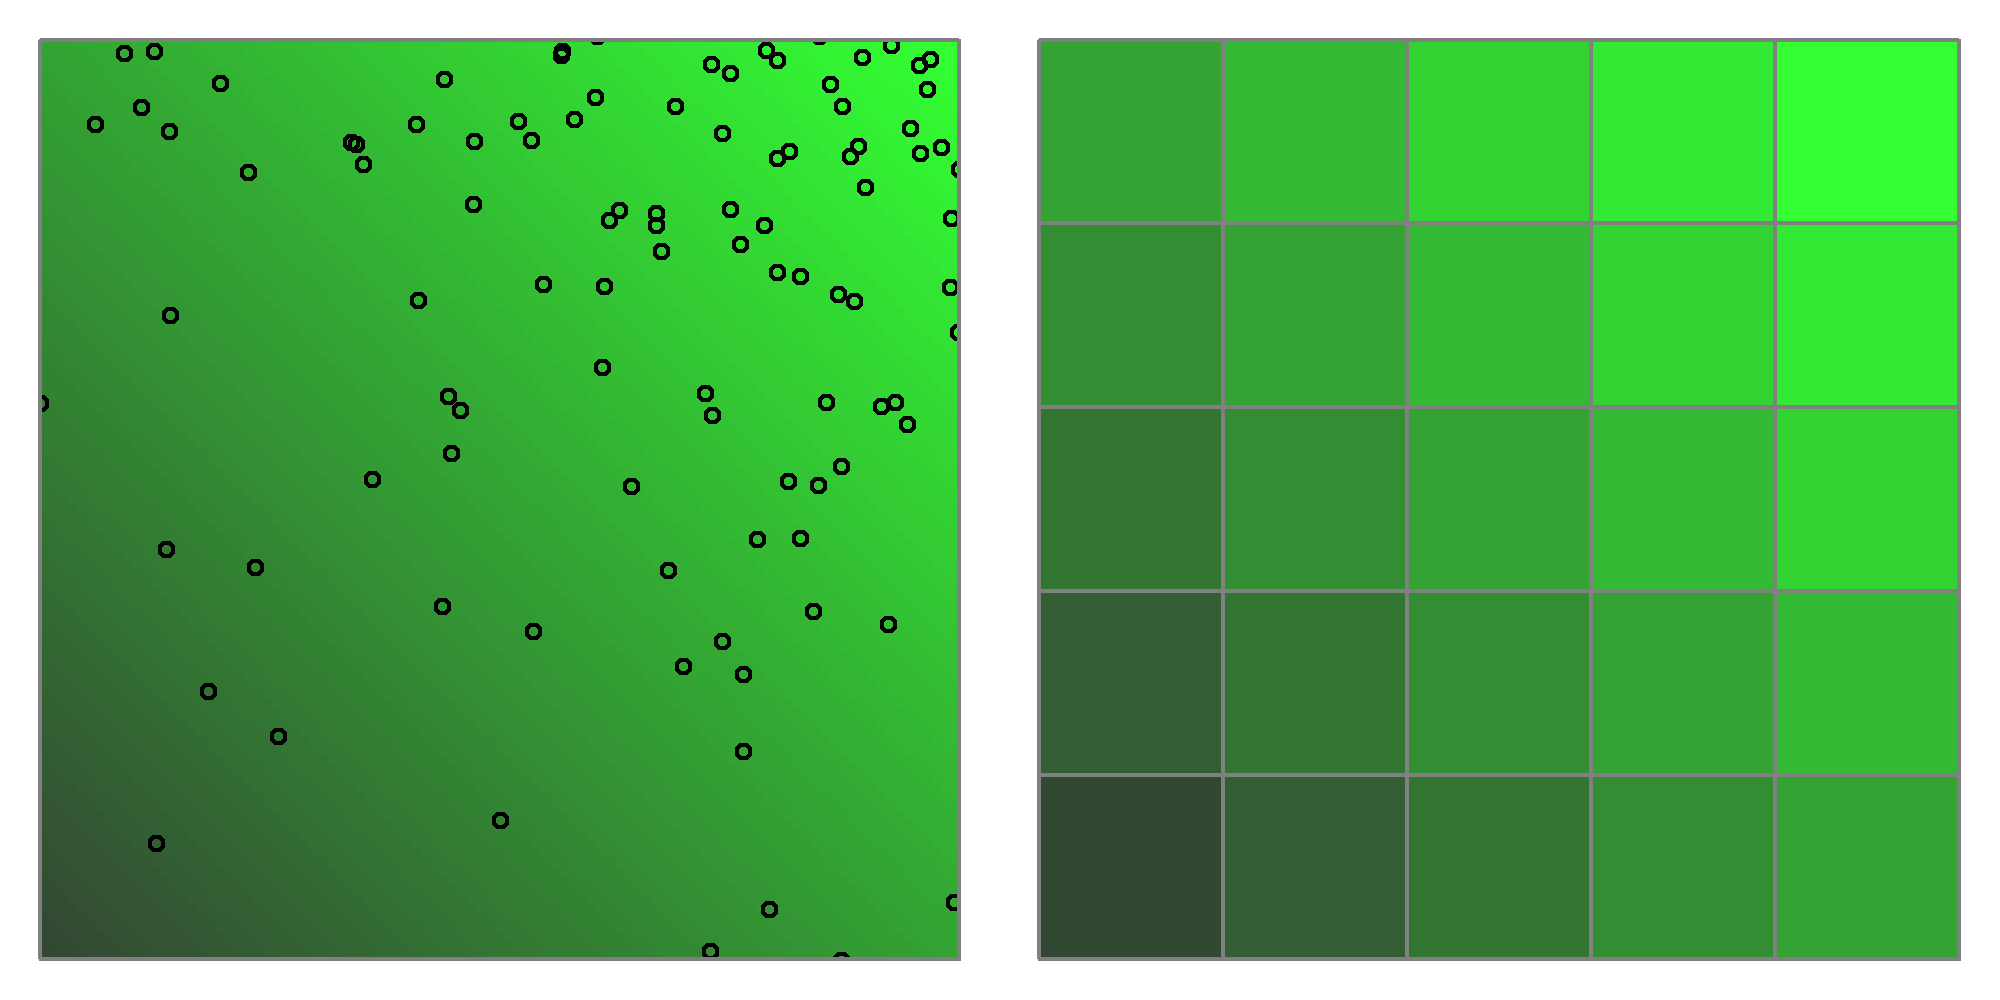
\includegraphics[width=\textwidth]{Ch11/figs/heteroPlots}
\label{state-space.fig.hetero}
\caption{An example of a spatial covariate, say elevation, and a
  realization from an inhomogeneous Poisson point process with
  and $\mu(\mathbf{s}, \bm{\beta}) = \exp(\beta_0 + \beta_1
  \mbox{ELEV}(\mathbf{s}))$ where $\beta_0=-6$ and $\beta_1=1$.}
\end{figure}

The 41 simulated points are shown in
Fig~\ref{state-space.fig.hetero}. High elevations
are represented by light gray and low elevations are darker. The
density of points in apparently higher in lighter regions
suggesting that these simulated animals prefer high
elevations.  %Perhaps they are mountain goats.
%The underlying model describing this preference is
%$\log(\mu(s)) = \exp(\beta \times elev(s))$
%where $\beta=2$ is the parameter to be estimated.
Given these points, we will now estimate $\beta_0$ and $\beta_1$ by
minimizing the negative-log-likelihood using \R's \verb+optim+
function.

\begin{small}
\begin{verbatim}
nll <- function(beta) { # negative log-likelihood
    beta0 <- beta[1]
    beta1 <- beta[2]
    EN <- cuhre(2, 1, mu, beta0=beta0, beta1=beta1)$value
    -(sum(beta0 + beta1*elev.fn(s)) - EN)
}
starting.values <- c(0, 0)
fm <- optim(starting.values, nll, hessian=TRUE)
cbind(Est=fm$par, SE=sqrt(diag(solve(fm$hessian)))) # estimates and SEs
\end{verbatim}
\end{small}

Maximizing the likelihood took a fraction of a second, and we
obtained estimates of $\hat{\beta}_0=-5.93$ and $\hat{\beta}_1=0.95$,
which are very close to the data generating values. The 95\% confidence
interval for $\hat{\beta}_1$ is [0.61, 1.3] and since it does not
include zero, the null hypothesis that $\beta_1=0$, i.e. that there is
no effect of elevation on density, can be rejected. In addition to testing
hypotheses, these results can be used to predict population size in
new regions or create predicted density surface maps by plugging the
parameter estimates into Eqs.~\ref{state-space.eq.loglin} and~\ref{state-space.eq.EN}.

This example demonstrates
that if we had the data we wish we had, i.e. if we knew the
coordinates of the activity centers, we could easily estimate the
parameters governing the underlying point process and make inferences
about spatial variation in density and abundance. Unfortunately, in
SCR, the activity centers cannot be directly observed; however,
spatial recaptures provide the information needed to
estimate these latent parameters.

\section{Fitting inhomogeneous point process SCR models}

\subsection{Continuous space}

% One of the nice things about hierarchical models is that they
% %allow us to
% break a complex problem up into a series of simpler conditional
% sub-models. The problem faced in the analysis of SCR data is that the
% underlying point process is not observed, and so an
% observation model is needed to describe how the observed data result from
% the latent activity centers. Thus, in SCR, we can simply add the methods described above into a likelihood
% function or an MCMC algorithm to simulate the posterior distributions of $\beta$ conditional on the
% simulated values of $\mathbf{s}$.

In this example, we will use the same set of points simulated in the
previous section to generate spatial capture-recapture
data. Specifically, we overlay a grid of 49
traps on the map shown in Fig.~\ref{state-space.fig.hetero} and
simulate capture histories conditional upon the activity
centers. Then, we will attempt to estimate the activity center
locations as though we did not know where they were, as is the case in
real applications. The following \R~code simulates encounter histories under a
Poisson observation model (see Chapt. \ref{chapt.poisson-mn}), which could be appropriate in camera
trapping studies or when using other methods in which animals could
be detected multiple times at a trap during a single occasion.

\begin{samepage}
\begin{small}
\begin{verbatim}
xsp <- seq(20, 80, by=10); len <- length(xsp)
X <- cbind(rep(xsp, each=len), rep(xsp, times=len)) # traps
ntraps <- nrow(X); noccasions <- 5
y <- array(NA, c(N, ntraps, noccasions)) # capture data
sigma <- 5  # scale parameter
lam0 <- 1   # basal encounter rate
lam <- matrix(NA, N, ntraps)
set.seed(5588)
for(i in 1:N) {
    for(j in 1:ntraps) {
        # The object "s" was simulated in previous section
        distSq <- (s[i,1]-X[j,1])^2 + (s[i,2] - X[j,2])^2
        lam[i,j] <- exp(-distSq/(2*sigma^2)) * lam0
        y[i,j,] <- rpois(noccasions, lam[i,j])
    }
}
# data augmentation
nz <- 80; M <- nz+nrow(y)
yz <- array(0, c(M, ntraps, K))
yz[1:nrow(y),,] <- y # Fill data augmentation array
\end{verbatim}
\end{small}
\end{samepage}

Now that we have a simulated capture-recapture dataset \texttt{y} and we have
augmented it to create the new data object \texttt{yz}, we can
estimate the parameters using MCMC.  A commented Gibbs sampler written
in \R~is available in the accompanying \R~package \scrbook~(see
\texttt{?scrIPP}). This function is not meant to be an all purpose
tool for fitting SCR models using MCMC---instead, it is presented so
that interested readers can better understand the computational
aspects of the problem and can modify it for their purposes.
The function can be used as so:
\begin{samepage}
  \begin{small}
\begin{verbatim}
set.seed(3434)
fm1 <- scrIPP(yz, X, M, 10000, xlims=c(0,100), ylims=c(0,100),
              space.cov=elev.fn,
              tune=c(0.4, 0.2, 0.3, 0.3, 7))
plot(mcmc(fm1$out))
\end{verbatim}
  \end{small}
\end{samepage}
which requests 10000 posterior samples and estimates the effect of the
spatial covariate, elevation, on density. Currently, the function
places uniform priors on the parameters $\sigma$, $\lambda_0$,
$\beta_0$ and $\beta_1$, although this could easily be modified. Note that any spatial
covariate that returns a real value for any location in the
state-space can be supplied using the \texttt{space.cov} argument. The resulting
trace plots of the Markov chains and the posterior distributions for
three parameters are
shown in Fig.~\ref{state-space.fig.fm1post}. The chains appear to
converge rapidly but may need to be run longer to reduce Monte Carlo
error.

\begin{figure}
  \centering
  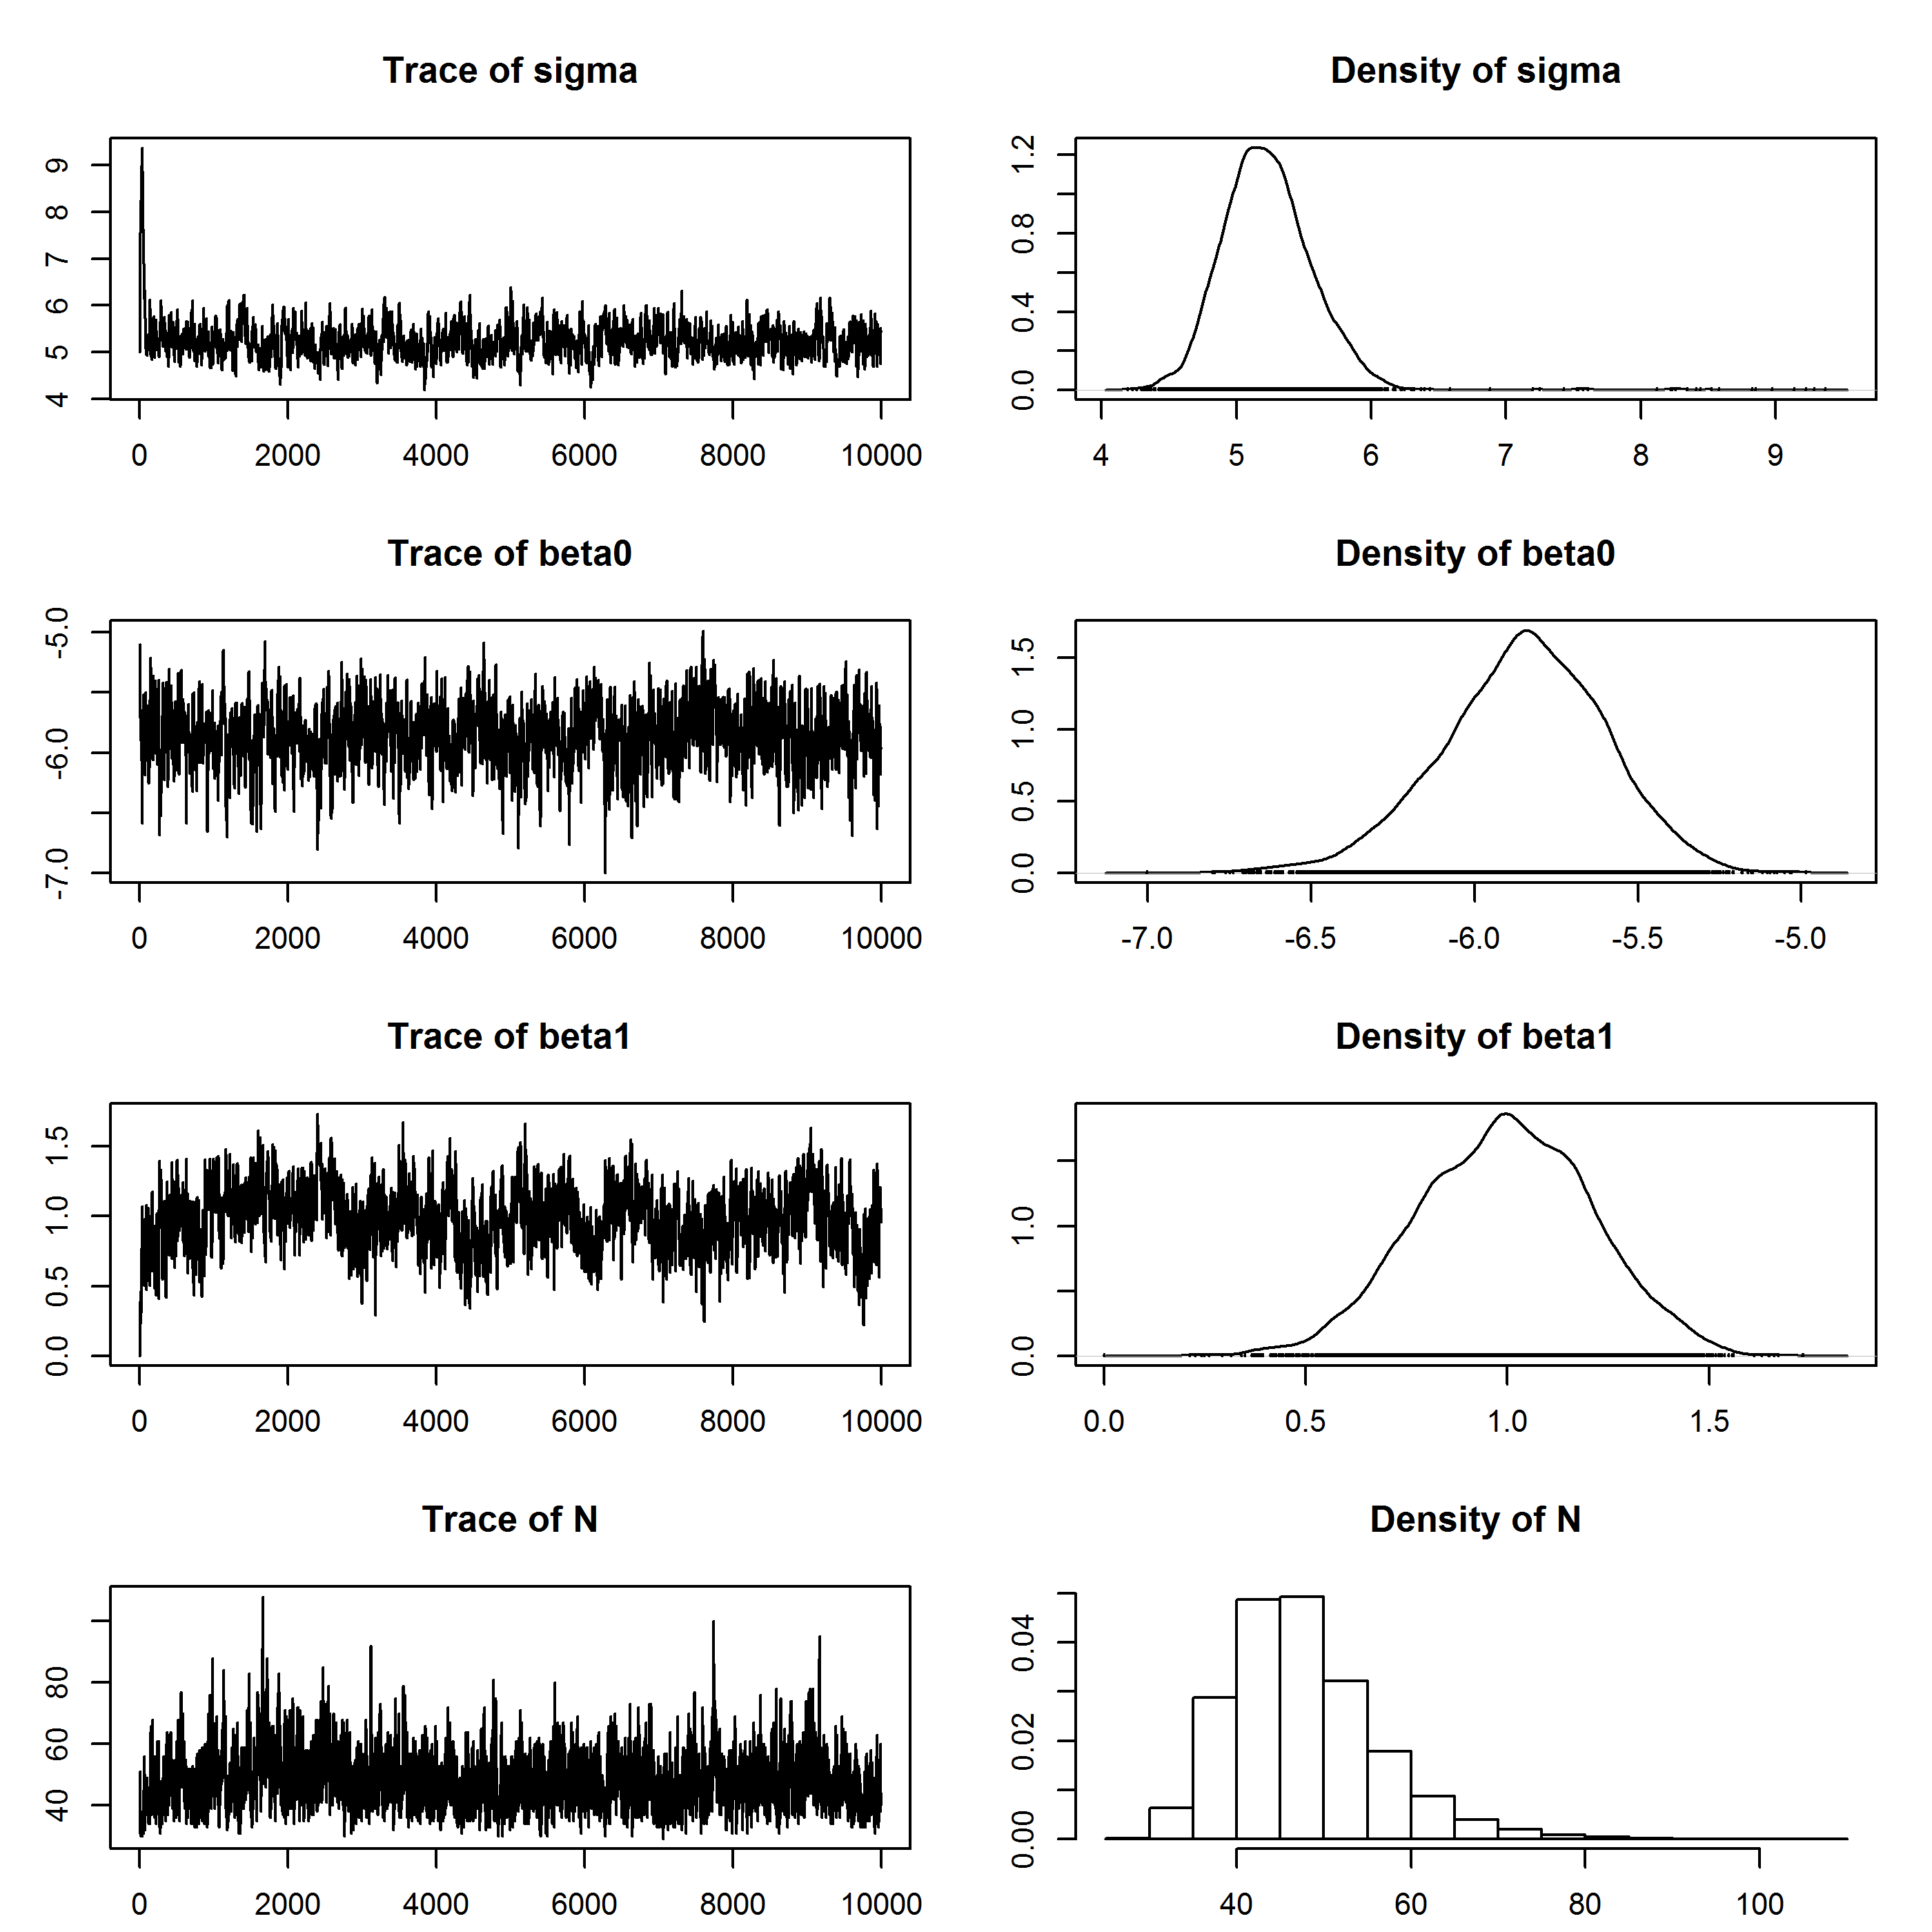
\includegraphics[width=0.8\textwidth]{Ch11/figs/fm1p}
  \caption{Trace plots and posterior distributions from MCMC analysis
    of SCR model with inhomogeneous point process. Analysis was
    conducted using the \texttt{scrIPP} function in the accompanying
    \R~package \scrbook.}
  \label{fig:state-space.fig.fm1post}
\end{figure}
%For comparison, we also fit this model using $\texttt{secr}$. See the
%help file \texttt{Ch-IPP} in \scrbook~ for \R~commands necessary to
%prepare the data for \secr.

\begin{table}%[b]
\centering
\caption{Summary of posterior distributions from SCR model with
  inhomogeneous point process. }
\begin{tabular}{lrrrr}
\hline
Parameter 	 	& Mean  	& SD    	& 2.5\% 	& 97.5\% \\
\hline
 $\sigma=5$ 	 	&  5.232 	&  0.310 	&  4.681 	&  5.858 \\
 $\lambda_0=1$ 	 	&  0.802 	&  0.119 	&  0.595 	&  1.049 \\
 $\beta_0=-6$ 	 	& -5.856        & 0.2542        & -6.376        & -5.393 \\
 $\beta_1=1$ 	 	&  0.985 	&  0.209 	&  0.575 	&  1.378 \\
 $N=41$ 	 	& 47.615 	&  8.041 	& 35.000 	& 66.000 \\
 $\mathbb{E}[N]=39.9$ 	& 47.551 	& 10.992 	& 29.837 	& 71.332 \\
\hline
\end{tabular}
\label{state-space.tab.simIPP}
\end{table}

Summaries of the posterior distributions are presented in
Table~\ref{state-space.tab.simIPP}. The posterior means for $\beta_0$
and $\beta_1$ are quite similar to MLEs from the analysis in the
previous section in which we assumed no observation error. However, we
see that the confidence intervals are wider. With respect to the other
parameters in the model, we see that all of the data
generating parameter fall within the 95\% credible intervals. One
interesting thing to note is that, although the point estimates for
the expected and realized values of $N$ are quite similar, the
estimate is more precise for the realized value. This is to be
expected because the uncertainty associated with the realized value of
$N$ is entirely determined by the encounter rate parameters. That is,
if we could perfectly detect all of the individuals in $\cal S$, there
would be no uncertainty about $N$. In contrast, the variance for
expected value of $N$ is affected by the variance of all the parameters
in the model, not just the encounter rate parameters. See
\citet{efford_fewster:2012} for additional discussion on the
difference between realized and expected values of abundance.
%, and we see that the point
%estimates and confidence/credible intervals are quite similar from the
%MCMC and maximum likelihood (ML) analyses. One exception is that the
%confidence intervals for $N$ and the expected value of $N$ are
%somewhat different. This may result from the fact that the MCMC
%analysis assumed a binomial prior for $N$, whereas the ML analysis
%assumed a Poisson prior.


Fitting continuous space inhomogenous point process models is somewhat
difficult in \bugs~because the ``IPP'' prior $[\mathbf{s}_i | \bm
\beta]$---unlike the uniform prior---is not one of the
available distributions that comes with the software. It is
possible to add new distributions in \bugs, but it is somewhat
cumbersome.  \secr~allows
users to fit continuous space models using linear or polynomial functions of the x- and y-
coordinates, but it does not accept truly continuous covariates that
are functions of space. However, these
are not really important limitations because discrete
space versions of the model are straight-forward, and virtually all spatial
covariates are, or can be, defined as such.

\subsection{Discrete space}
\label{modeling.sec.discrete}

To fit inhomogeneous point process models using covariates in discrete
space, i.e. in raster format, we follow the same steps
as outlined in Chapter~\ref{chapt.poisson-mn}---we define ${\bf s}_i$ as
pixel ID, and we use the categorical distribution as a prior. This
effectively changes the problem from estimating the coordinates of an
activity center, to estimating the pixel in which an activity center is
located. As pixel size approaches zero, these two become equivalent. A good
example is found in \citep{mollet_etal:2012}. Here we present
an analysis of the simulated data shown in the %right panel of
Fig.~\ref{state-space.fig.hetero}. The spatial covariate, let's call it
forest canopy height (CANHT), was simulated
using using the code shown on the help page
\verb+ch11+ in \scrbook. The points are the number of
activity centers in each pixel, generated from a single realization of
the inhomogeneous point process model with intensity
$\mu(x, \bm{\beta}) = \exp(\beta_0 + \beta_1 \text{CANHT}(s))\times\text{pixelArea}$,
where $\beta_0 = -6$ and $\beta_1 = 1$.
\begin{figure}[ht]
\centering
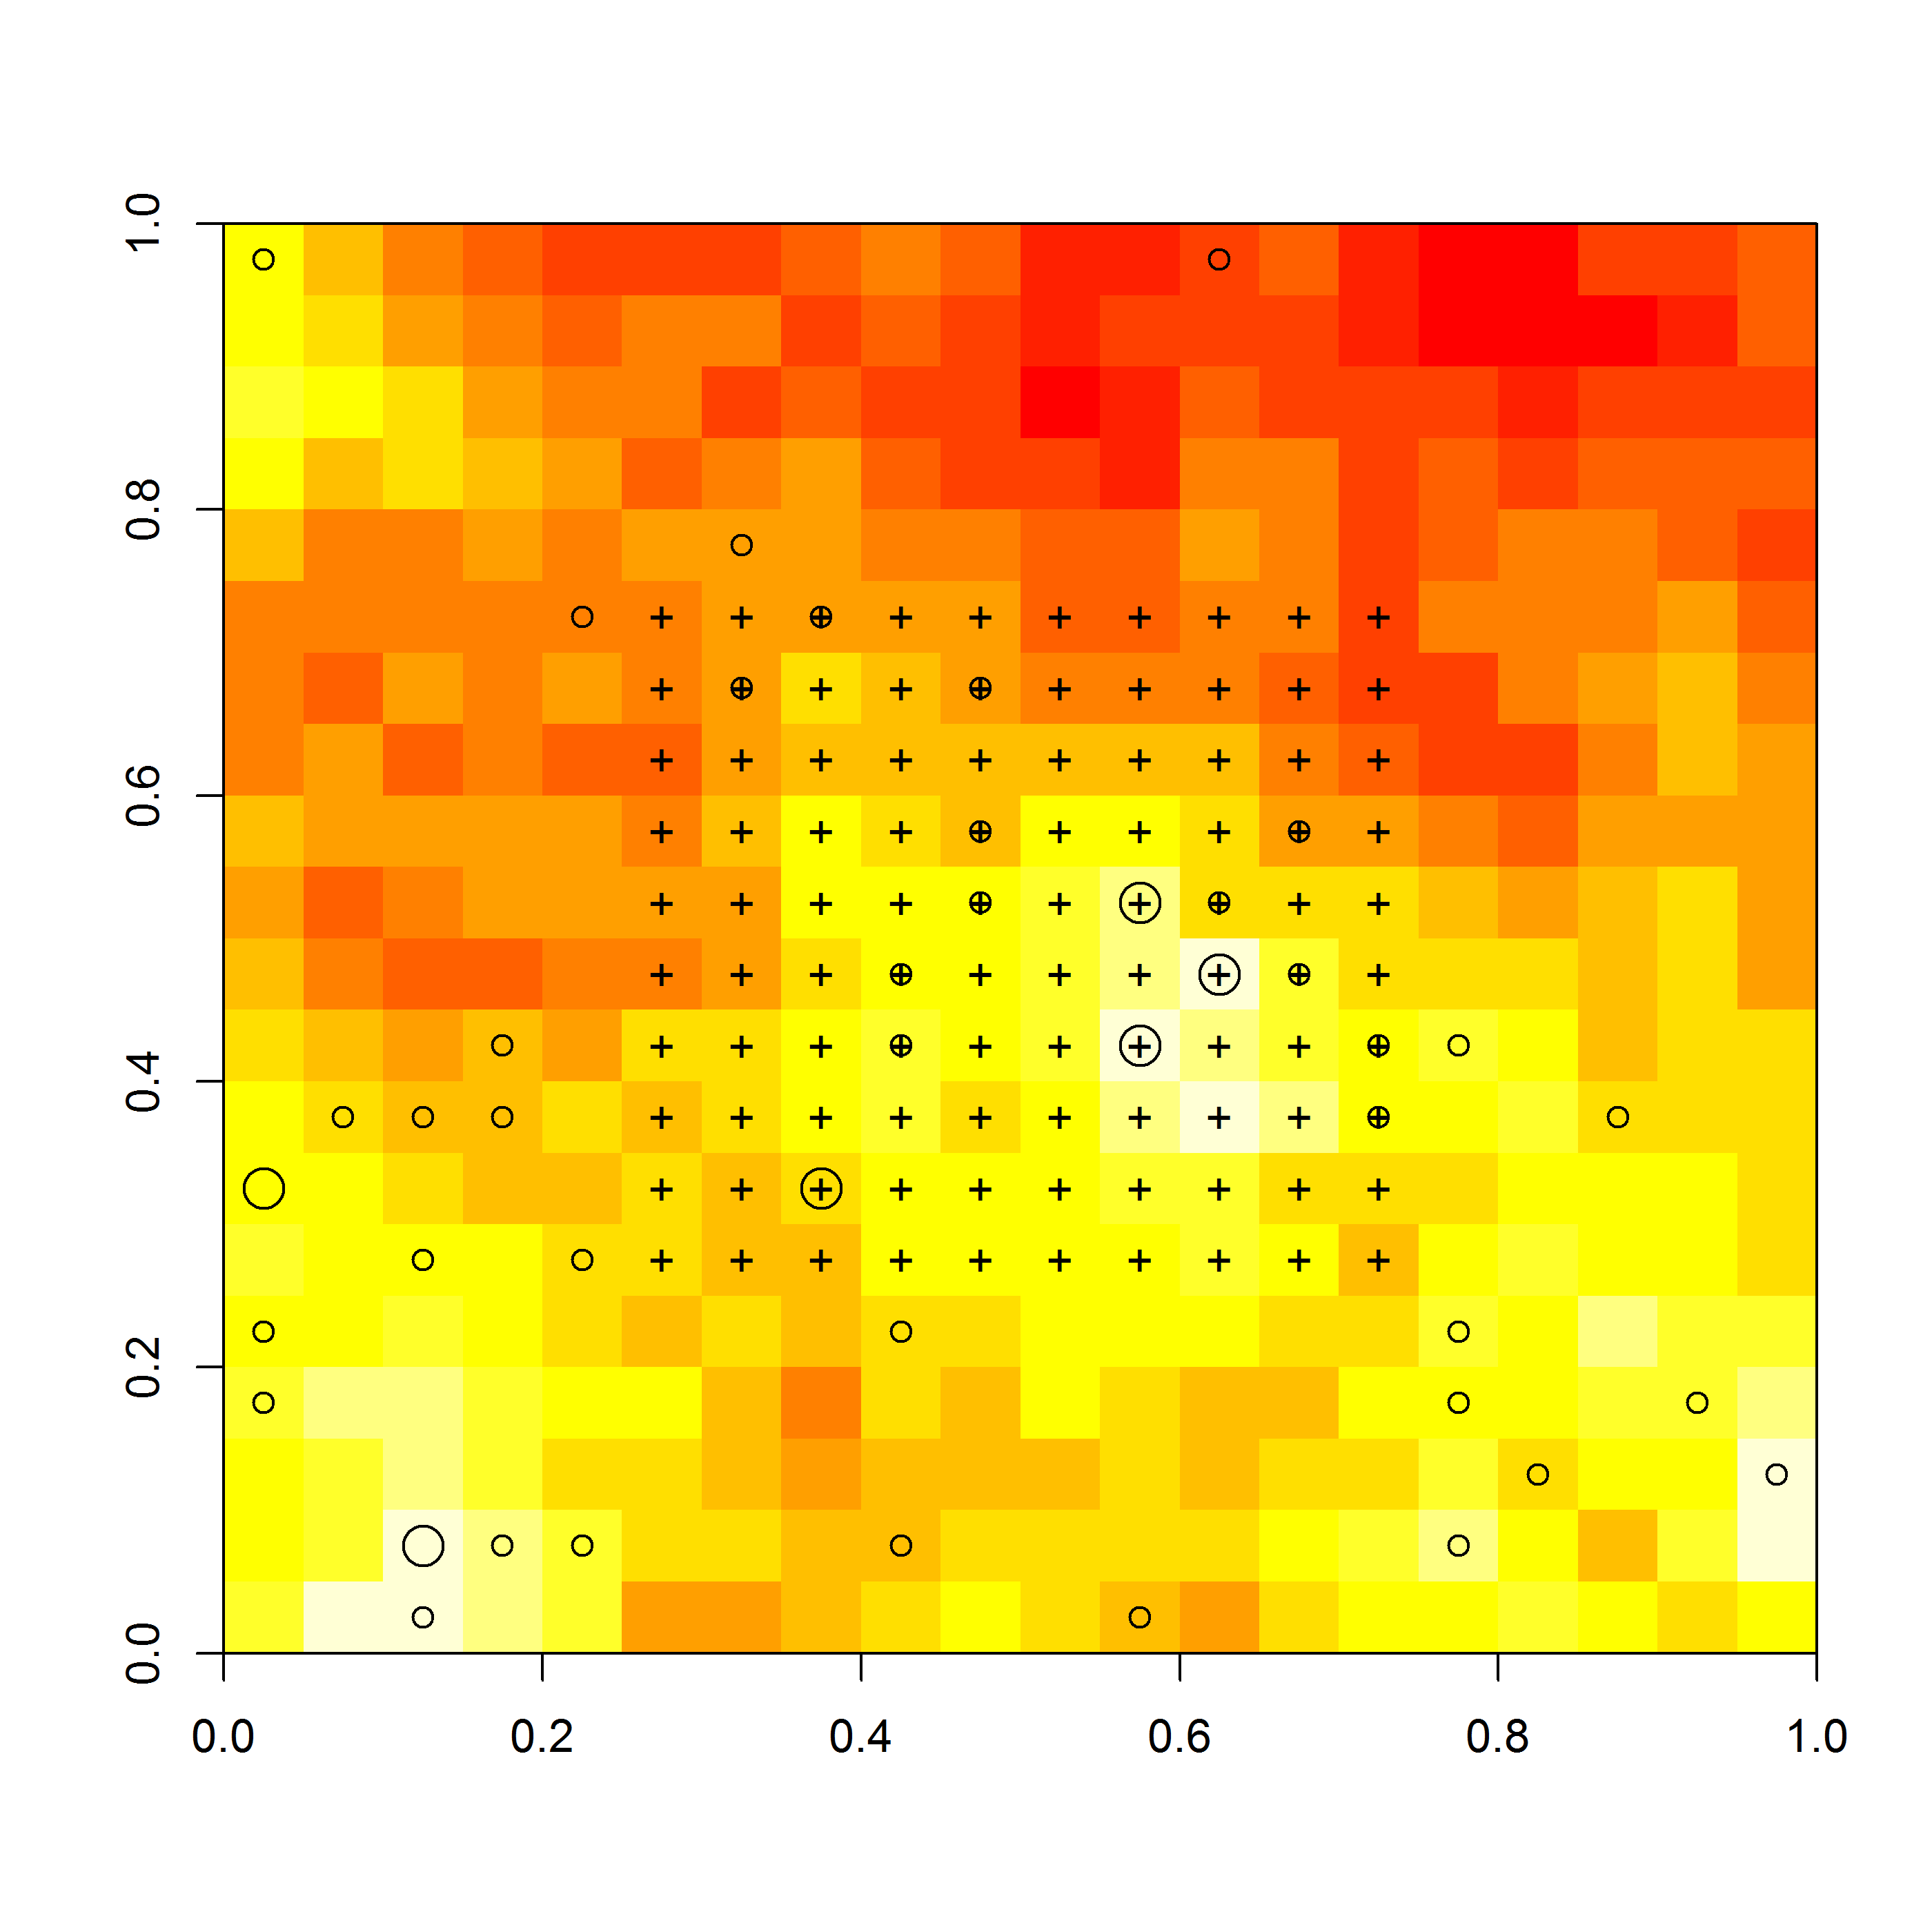
\includegraphics[width=0.6\textwidth]{Ch11/figs/discrete}
\label{ch9.fig.discrete}
\caption{Simulated activity centers in discrete space. The spatial
  covariate, canopy height, is highest in the lighter areas. Density of
  activity centers (circles) increases with elevation. A single
  activity center is shown as a small circle, and larger circles
  represent two activity centers in a pixel. Trap locations
  are shown as crosses.}
\end{figure}

The \bugs~description of the model is shown in
panel~\ref{ch9.panel1}. The vector \verb+probs[]+ is the prior
probability defined
by Eq.~\ref{state-space.eq.pdf.hetero.d}, which is the probability that an individual's
activity center is located at pixel $\bf s$. \verb+Sgrid+ is the
matrix of coordinates for each pixel.

\begin{panel}%[h!]
\centering
\rule[0.15in]{\textwidth}{.03in}
\begin{small}
\begin{verbatim}
model{
sigma ~ dunif(0, 20)
lam0 ~ dunif(0, 5)
beta0 ~ dunif(-10, 10)
beta1 ~ dunif(-10, 10)
for(j in 1:nPix) {
  mu[j] <- exp(beta0 + beta1*CANHT[j])*pixArea
  probs[j] <- mu[j]/EN
}
EN <- sum(mu[]) # Expected value of N, E[N]
psi <- EN/M
for(i in 1:M) {
  w[i] ~ dbern(psi)
  s[i] ~ dcat(probs[])
  x0g[i] <- Sgrid[s[i],1]
  y0g[i] <- Sgrid[s[i],2]
  for(j in 1:ntraps) {
    dist[i,j] <- sqrt(pow(x0g[i]-traps[j,1],2) + pow(y0g[i]-traps[j,2],2))
    lambda[i,j] <- lam0*exp(-dist[i,j]*dist[i,j]/(2*sigma*sigma)) * w[i]
    y[i,j] ~ dpois(lambda[i,j])
    }
  }
N <- sum(w[]) # Realized value of N
}
\end{verbatim}
\end{small}
\rule[0.15in]{\textwidth}{.03in}
\caption{\bugs~code for fitting inhomogeneous point process model in
  discrete space.}
\label{ch9.panel1}
\end{panel}

This model can also be fit in \secr, which refers
to the raster data as a ``habitat mask''. \R~code to format the data
and fit the models using \secr~and \jags~is available in \scrbook---see
\verb#help(ch9secrYjags)#. Results of the
comparison are shown in Table \ref{state-space.tab.jagsVsecr} and are
very similar as expected. The differences that do exist can be
explained by a variety of reasons. For one, there exists some Monte
Carlo error in the Bayesian posterior summaries. There is also the
fact that posterior summaries can be computed in numerous ways---for
example, we could have presented posterior modes or medians instead of
means---or, we could have shown highest posterior density credible
intervals instead of simple percentiles. The posteriors would also
differ if we chose more informative priors than the uniform
distributions used here. We see no reason why these
issues should be seen as limitations of the Bayesian analysis, rather
we would argue that the posterior distribution, which describes the
probability that the parameter equals any particular value, is a
better descriptor undertainty than any particular point estimator or
confidence interval. Futhermore, most of these differences are minor,
and hardly worth mention. The only exception is that the estimates of
the expected and realized values of $N$ are closer to the data
generating values in the Bayesian analysis, and the Bayesian credible
intervals are narrower than the frequentist confidence intervals. This
is likely a result of the fact that the Bayesian analysis assumed
that $N$ was binomial whereas the frequentist analysis
assumed a Poisson prior for $N$, and the variance of the binomial will
always be less than or equal to the variance of Poisson distribution
for a shared expectation.

\begin{table}%[h!]
\centering
\caption{Comparison of \secr~and \jags~results. Point estimates from
  the Bayesian analysis are posterior means. Intervals are lower and
  upper 95\% CIs.}
\begin{tabular}{lrlrrrr}
\hline
Par 	& Truth 	& Software 	& Mean 	& SD 	& 2.5\% & 97.5\% \\
\hline
$\lambda_0$ 	&  1.00 	& \textbf{JAGS} 	&  1.09 	& 0.11 	&  0.88 	&  1.33 \\
 $\lambda_0$ 	&  1.00 	& \texttt{secr} 	&  1.25 	& 0.13 	&  1.02 	&  1.54 \\
 $\sigma$ 	&  5.00 	& \textbf{JAGS} 	&  5.15 	& 0.23 	&  4.73 	&  5.63 \\
 $\sigma$ 	&  5.00 	& \texttt{secr} 	&  4.73 	& 0.20 	&  4.35 	&  5.15 \\
 $\beta_1$ 	&  2.00 	& \textbf{JAGS} 	&  3.59 	& 0.31 	&  2.96 	&  4.17 \\
 $\beta_1$ 	&  2.00 	& \texttt{secr} 	&  2.65 	& 0.31 	&  2.04 	&  3.26 \\
 $N$ 	& 53.00 	& \textbf{JAGS} 	& 39.14 	& 2.14 	& 36.00 	& 44.00 \\
 $N$ 	& 53.00 	& \texttt{secr} 	& 45.52 	& 4.34 	& 40.06 	& 58.31 \\
 $\mathbb{E}[N]$ 	& 49.00 	& \textbf{JAGS} 	& 38.83 	& 5.70 	& 28.49 	& 50.79 \\
 $\mathbb{E}[N]$ 	& 49.00 	& \texttt{secr} 	& 45.52 	& 8.02 	& 32.31 	& 64.13 \\
\hline
\end{tabular}
\label{state-space.tab.jagsVsecr}
\end{table}


\section{Ecological Distance and Density Covariates}

Habitat characteristics that affect spatial variation in density can also affect
home range size and movement behavior. For example, a
species that occurs at high density in a forest may be reluctant to
venture from a forest patch into an adjacent field. Thus, even if a
trap placed in a field is located very close to an animal's activity
center, the probability of capture may be very
low. In this case,  we could say that forest cover is a covariate of
both density and encounter probability,
and we could model it as such by combining the methods described in
this chapter with those described in Chapter~\ref{chapt.ecoldist}.

To demonstrate, we continue with our analysis of the data shown in
Fig~\ref{state-space.fig.hetero}. Once again, we suppose that density
increases with elevation, but this time, we also make the
assumption that home range size decreases as density increases. This
commonly-observed phenomenon can be explained by numerous factors such
as intra-specific competition \citep{sillett_etal:2004} or optimal
foraging behavior \citep{tufto_etal:1996,said_servanty:2005}. To model
this effect, we
introduce the parameter $\theta$, which determines the ``cost'' of
moving between pixels. If $\theta=0$, then the animal perceives
distance as Euclidean. If $\theta>0$, then least-cost distance (LCD)
is greater than than Euclidean distance (ED). In most cases, we would
not expect,
or should not even consider the possibility of $\theta<0$ because this
implies that LCD$<$ED, which would mean that an animal could view
1000km as 1m. In addition to the fact that this is not biologically
justifiable, it also suggests that the area of the state-space could
be infinitely large. Thus, one may want to enforce the constraint that
$\theta$ is strictly $\geq 0$. See Chapter~\ref{chapt.ecoldist} for
more details.

A question that arises is: Is possible to estimate $\bm \beta$
and $\theta$ using standard SCR data? In other words, can we model
spatial variation in density and connectivity at the same time,
using standard SCR data? Currently, it is not possible to
model least-cost distance using \jags~or \secr, so we wrote our own
function, \verb+scrDED+, to fit the model using maximum likelihood. An
example analysis is provided on the help page for the function in our
\R~package \scrbook. We briefly note here that the function requires
the capture history data, the trap locations, and the raster data
formatted using the {\tt raster} package
\citep{hijmans_vanetten:2012}. The linear model for the
intensity parameter $\mu(\mathbf{s}, \beta)$ and the least-cost distance
function $\text{lcd}(\theta)$ are specified using \R's formula interface. A
simple function call is
\begin{verbatim}
fm <- scrDED(y, traplocs=X, den.formula=~elev, dist.formula=~elev,
             rasters=elev.raster)
\end{verbatim}
To assess the possibility of estimating both $\bm \beta$ and $\theta$, we
conducted a small simulation study, generating 500 datasets from the
model with both parameters set to 1, which corresponds to the
conditions described above. The results indicate that it is
possible to estimate both parameters
(Fig~\ref{ch9.fig.sim}).

\begin{figure}[ht]
\centering
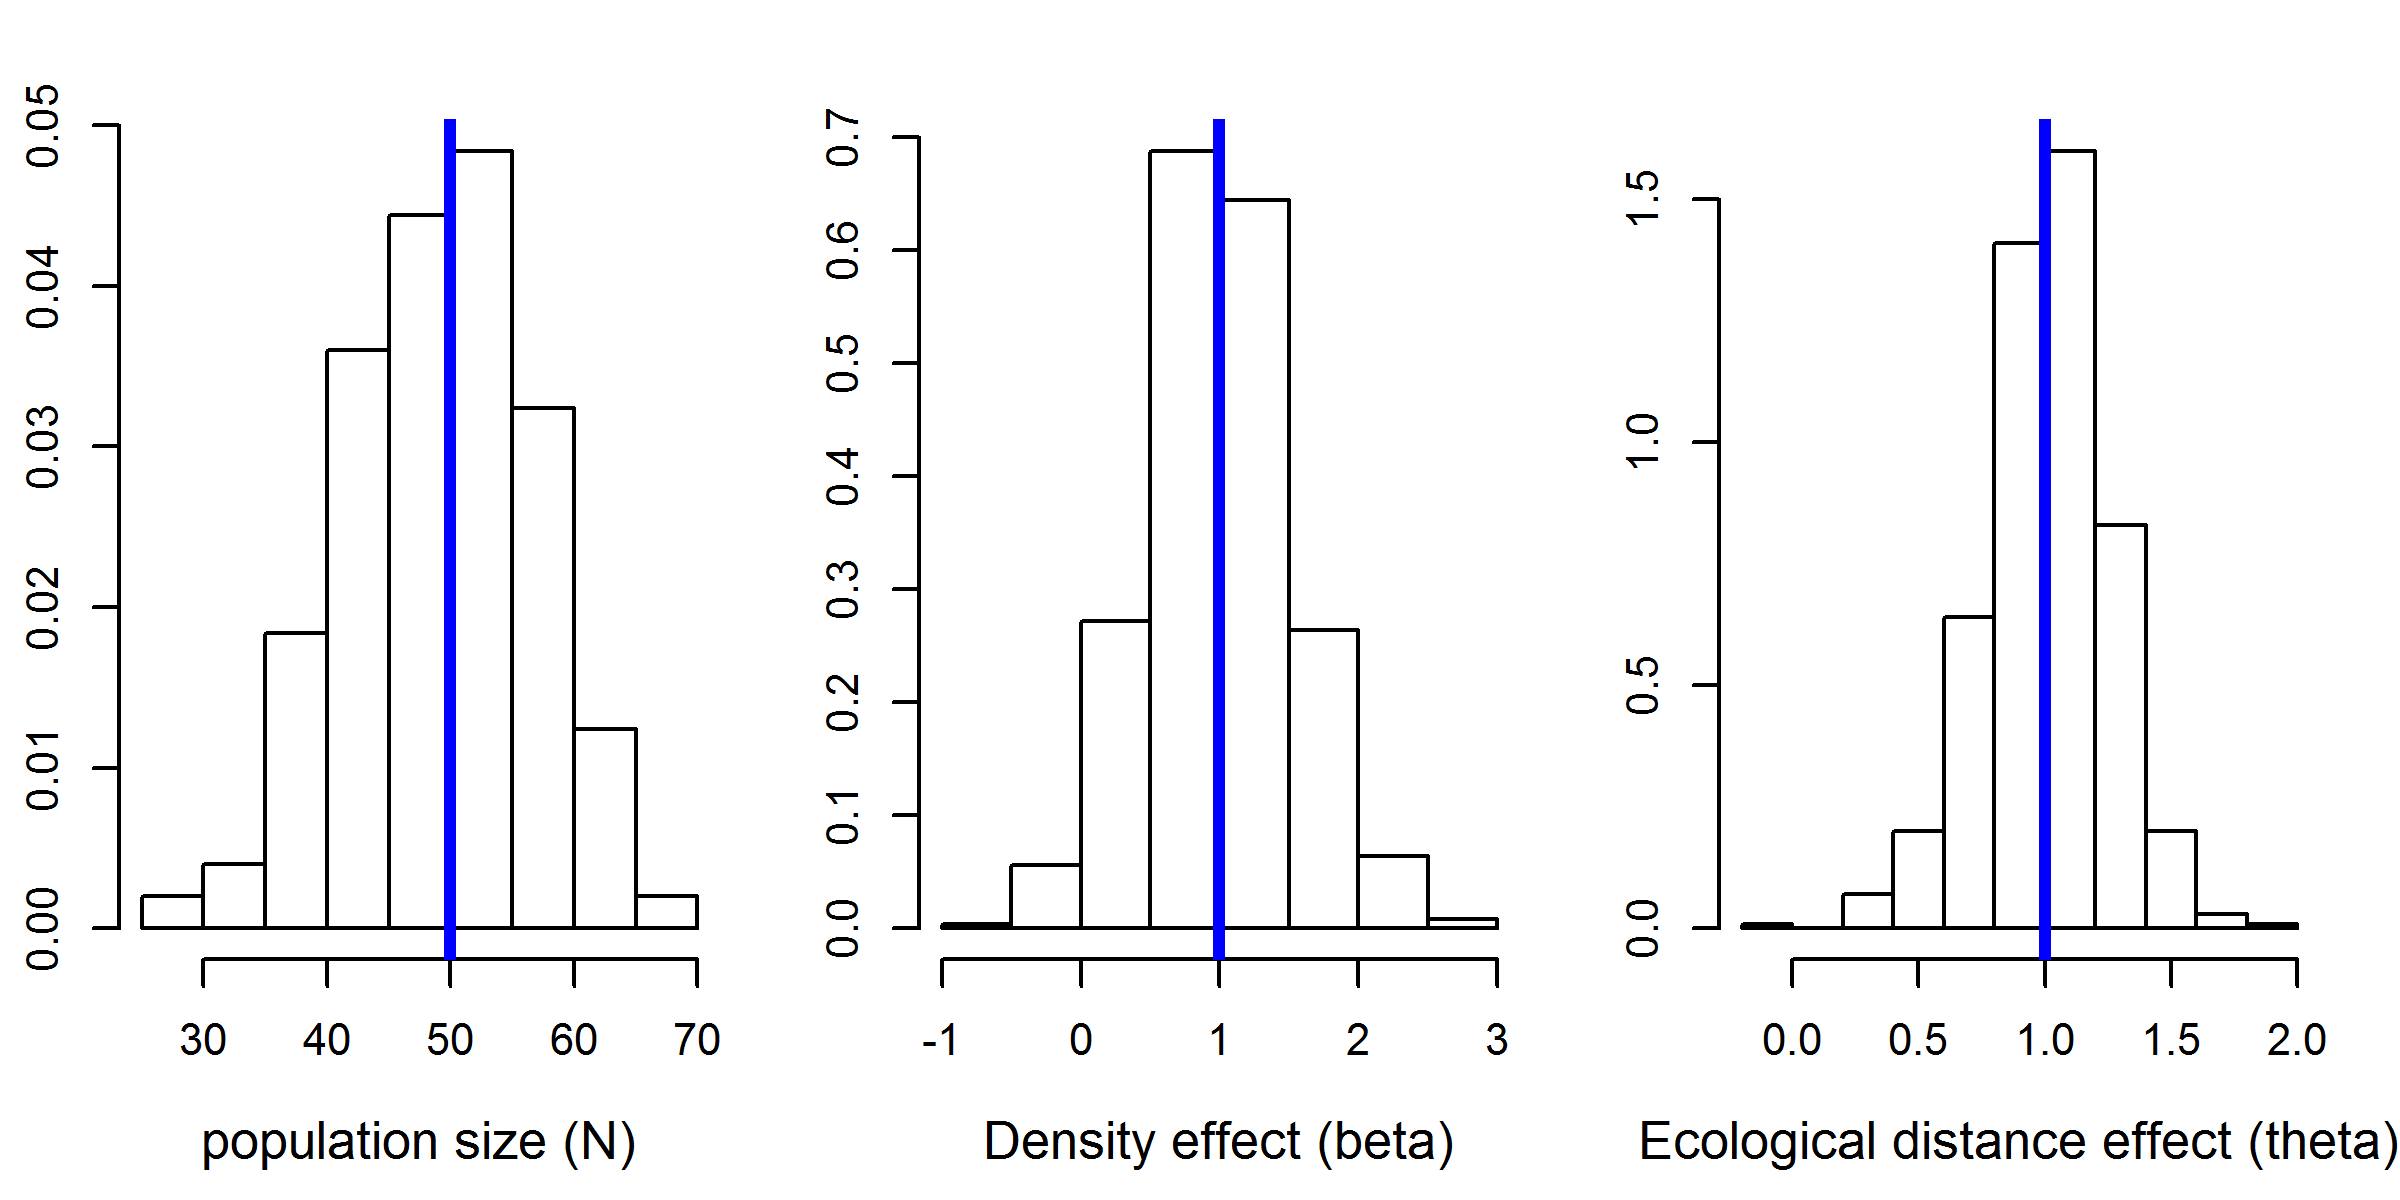
\includegraphics[width=4in,height=2in]{Ch11/figs/scrDEDsim}
\caption{Histograms of parameter estimates from 500 simulations under
  the model in which both density and ecological distance are affected
by the same covariate, elevation. The vertical lines indicate the
data-generating value.}
\label{ch9.fig.sim}
\end{figure}




\section{The Jaguar Data}

Estimating density of large felines has been a priority for many
conservation organizations, but no robust methodologies existed before
the advent of SCR. Distance sampling is not feasible for such rare and
cryptic species, and traditional capture-recapture methods yield
estimates that are highly sensitive to the subjective choice of the
effective survey area. In this example, we
demonstrate how readily density can be estimated for a
globally imperiled species using SCR. Furthermore, we show how
inhomogeneous point process models can be used to test important
hypotheses regarding the ecological factors affecting density.

In this example, we make use of a single year of data from an 8-year
camera-trapping study of jaguars in Argentina,
along the borders with Brazil and Paraguay. The data come from 46
camera stations, each consisting of a pair of cameras placed along
roads or trails. Forty-five detections of 16 jaguars (8 males and 8
females) were made over a 95-day sampling period. The mean number of
sampling days at each camera station was 48.2.

Estimating density is a central objective of this study because
ultimately, an estimate of the total population size for the entire
study area is needed, which can only be obtained by extrapolation of
density estimates. A second, and related, objective was to assess
the influence of poaching on jaguar density. Although jaguars
themselves are occasionally killed by poachers, the larger concern is
the influence of poaching on prey species. To protect jaguars and
related species, protected areas have
been established and three levels of protection are
recognized in the study region as depicted in Fig.~\ref{ch9.fig.jaguarCts}.

\begin{figure}[ht]
\centering
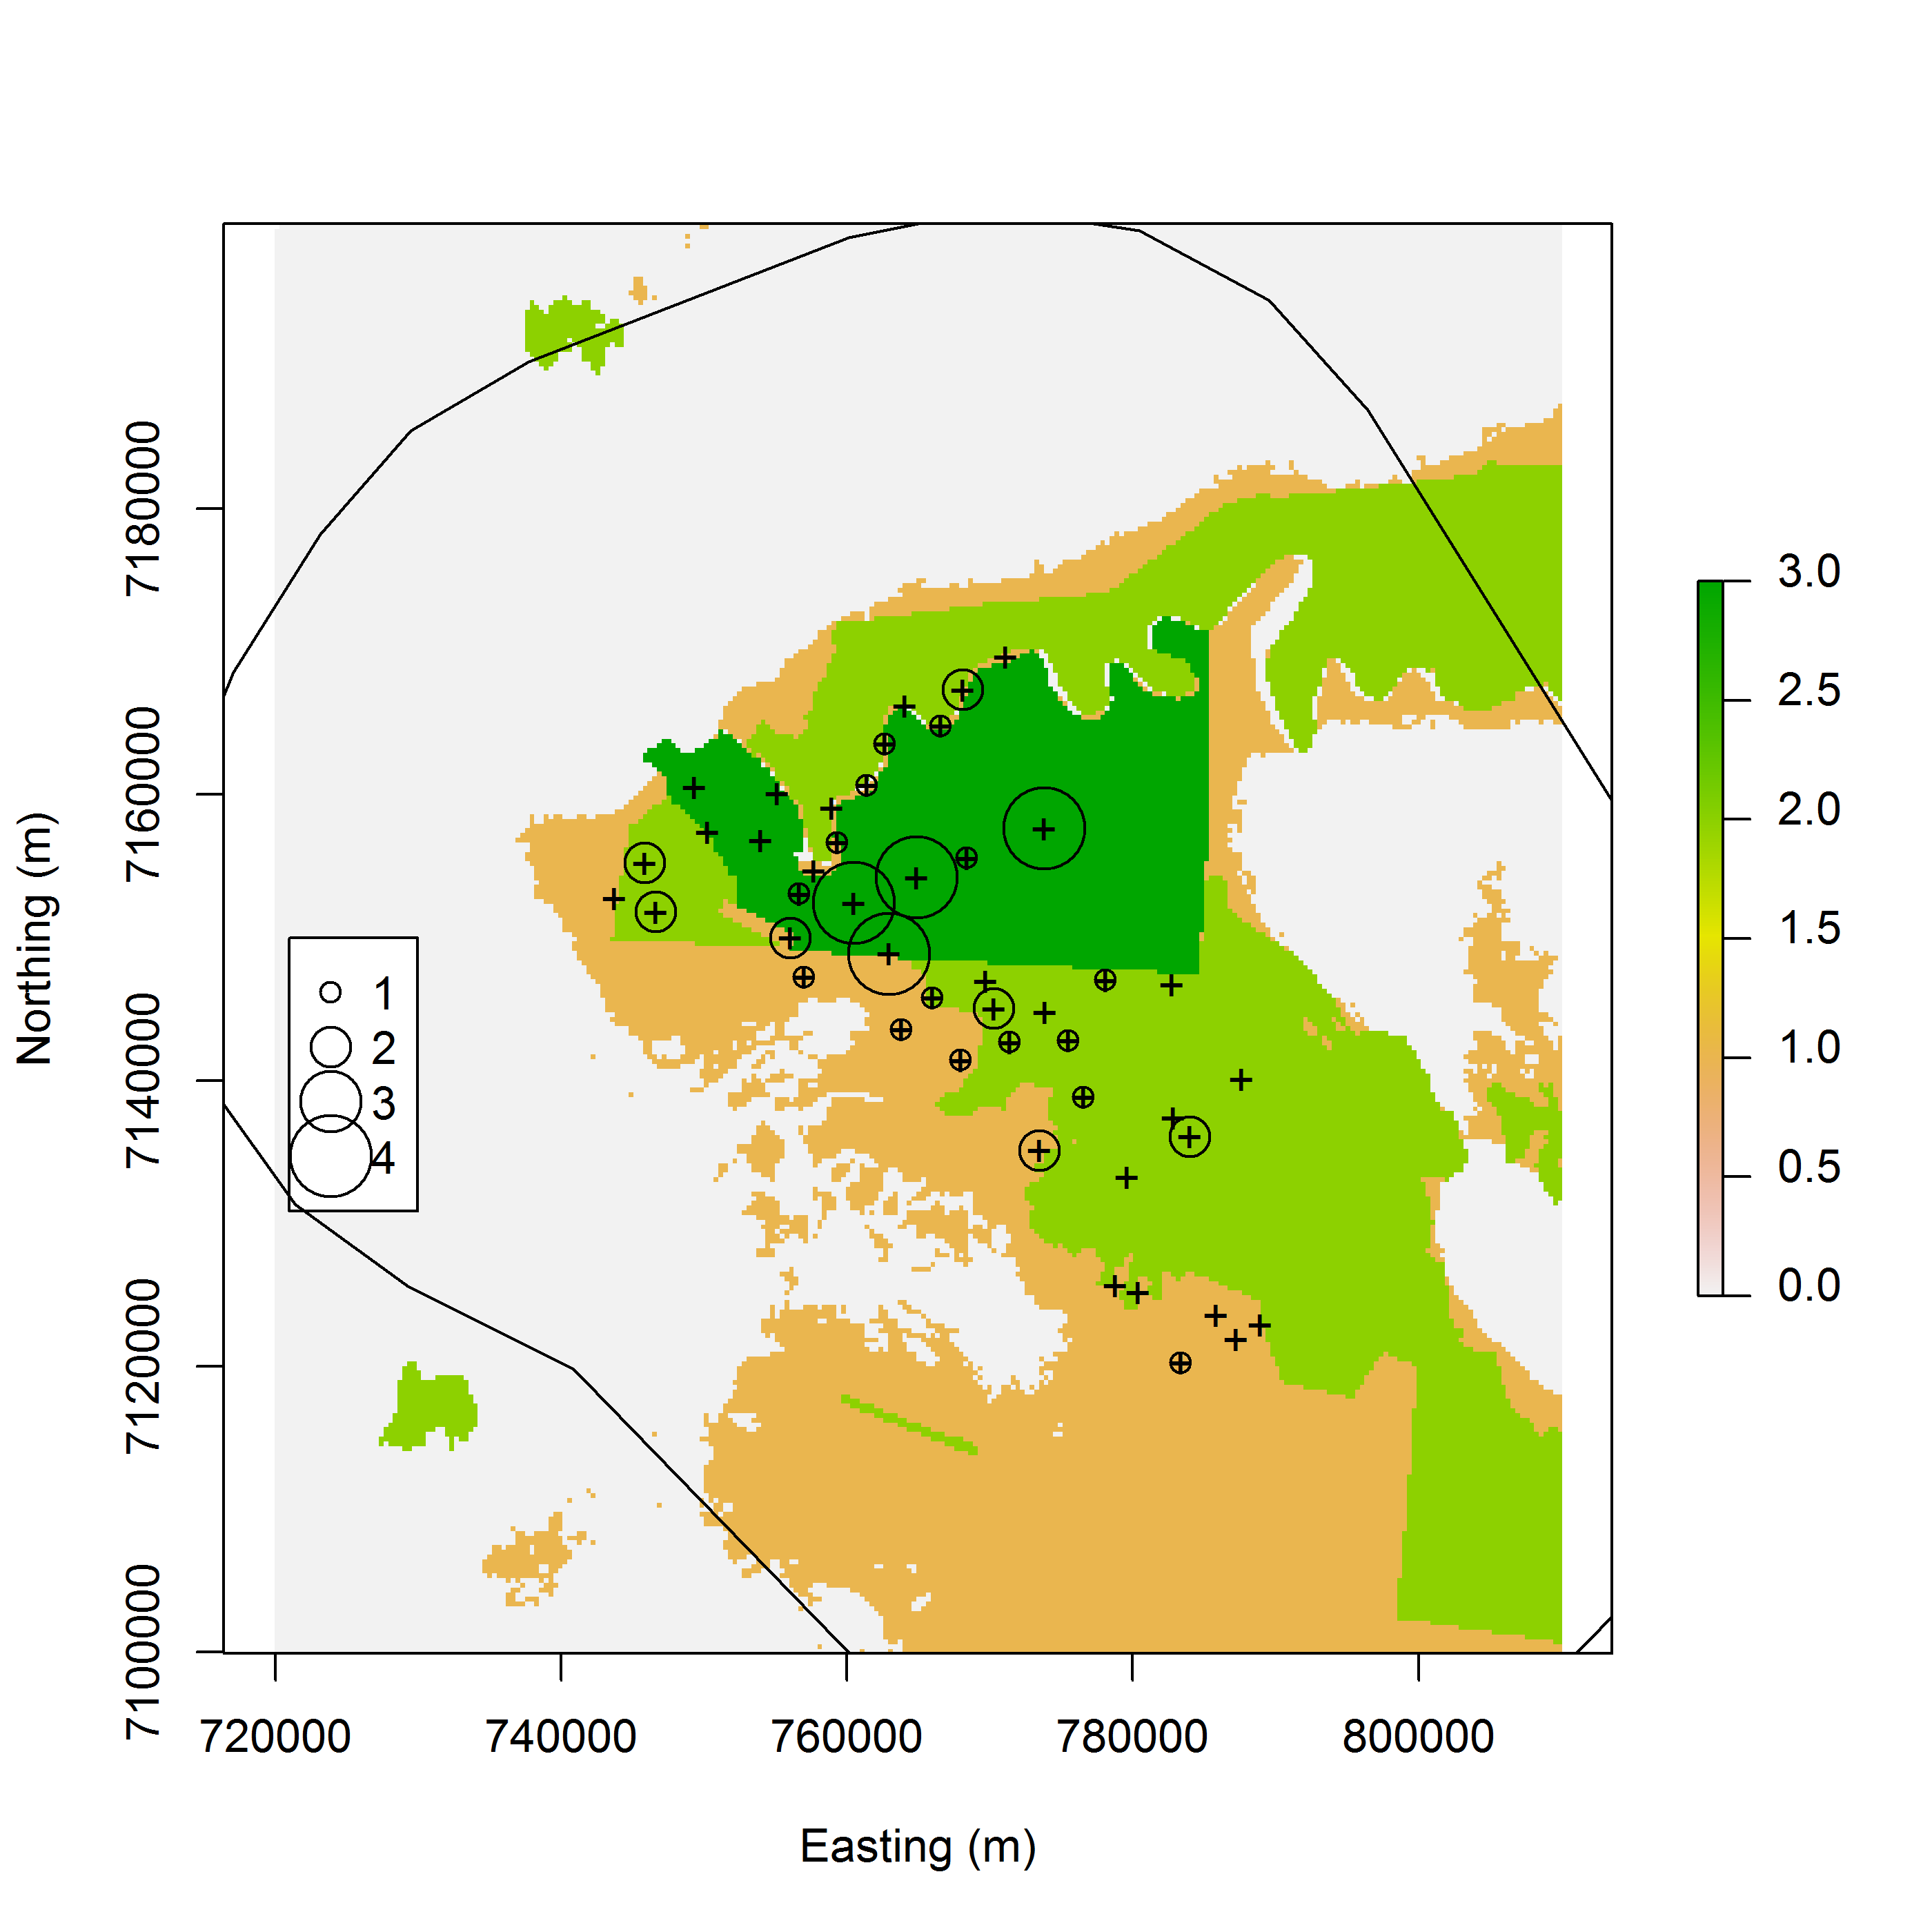
\includegraphics[width=3in,height=3in]{Ch11/figs/jaguarCountMap}
\label{ch9.fig.jaguarCts}
\caption{Jaguar detections at 46 camera trap stations. The three levels of
  protection status are no protection (beige), some protection (light
  green), and national park (dark green). Non-habitat is shown in gray
  and represents large soybean monocultures. }
\end{figure}

To assess the influence of poaching on jaguar density, we treated
protection status as an ordinal variable with 3 levels: no protection,
some protection, and high protection (national parks). Clearly these
are ordered, and our
hypothesis is that poaching pressure should decrease and jaguar
density should increase with the level of
protection. Thus, $\beta$ in this example is a ``slope''
parameter describing the degree to which protection status affects
jaguar density. We also hypothesized that males would have larger home
ranges than females \citep{conde_etal:2010,sollmann_etal:2011} and that the sex ratio may not be
1:1. Furthermore, we restricted the state-space to exclude the large
soybean monocultures surrounding the study area, and we only
considered
area south of the Iguazu River, which runs along the northern border
of the park shown in dark green in
Fig.~\ref{ch9.fig.jaguarCts}. Rather than restricting the
state-space, we could have modeled the permeability of the river using
the methods described in the previous section and in
Chapter~\ref{chapt.ecoldist}; however, no sampling was conducted on
the northern side of the river, and ancillary data indicates that
jaguars very rarely forge the waterway. \R~code to fit the model is
available in \scrbook  on the help page \verb+jaguarDataCh9+. Parameter
estimates are shown in Table\ref{ch9.tab.jagposts}.
\begin{table}
\centering
\caption{Summaries of posterior distributions from the model of jaguar
  density. $\sigma_f$ and $\sigma_m$ are the scale parameters of
  the half-normal detection function for females and males
  respectively. $\rho$ is the
  sex-ratio. $\lambda_0$ is base-line encounter rate. $\beta$ is the
  effect of protection on jaguar density. D is the overall density
  estimate. D1, D2, and D3 are the density estimates
  (jaguars/100km$^2$) for the three levels of protection. }
\begin{tabular}{lrrrrr}
\hline
& Mean & SD & 2.5\% & 50\% & 97.5\% \\
\hline
 $\sigma_f$ &  7361.731 &  1907.566 &  4899.740 &  7002.770 & 12083.110 \\
 $\sigma_m$ &  8177.068 &  1545.717 &  5916.151 &  7955.788 & 11842.486 \\
 $\rho$ &     0.516 &     0.118 &     0.286 &     0.516 &     0.741 \\
 $\lambda_0$ &     0.007 &     0.002 &     0.003 &     0.007 &     0.012 \\
 $\beta$ &     4.405 &     1.443 &     2.553 &     4.143 &     7.775 \\
 D &     0.533 &     0.708 &     0.000 &     0.000 &     0.072 \\
 D1 &     0.132 &     0.010 &     0.095 &     0.095 &     0.616 \\
 D2 &     1.415 &     0.050 &     0.214 &     0.531 &     1.503 \\
 D3 &     3.516 &     0.000 &     0.292 &     3.105 &     4.220 \\
\hline
\end{tabular}
\label{ch9.tab.jagposts}
\end{table}

Our results
indicate that efforts to protect jaguars by reducing poaching are
working. Density was $>$26 times higher in the national park than in the
unprotected area. Fig.~\ref{ch9:fig:Dsurface} shows the estimated
density surface.

\begin{figure}[ht]
\centering
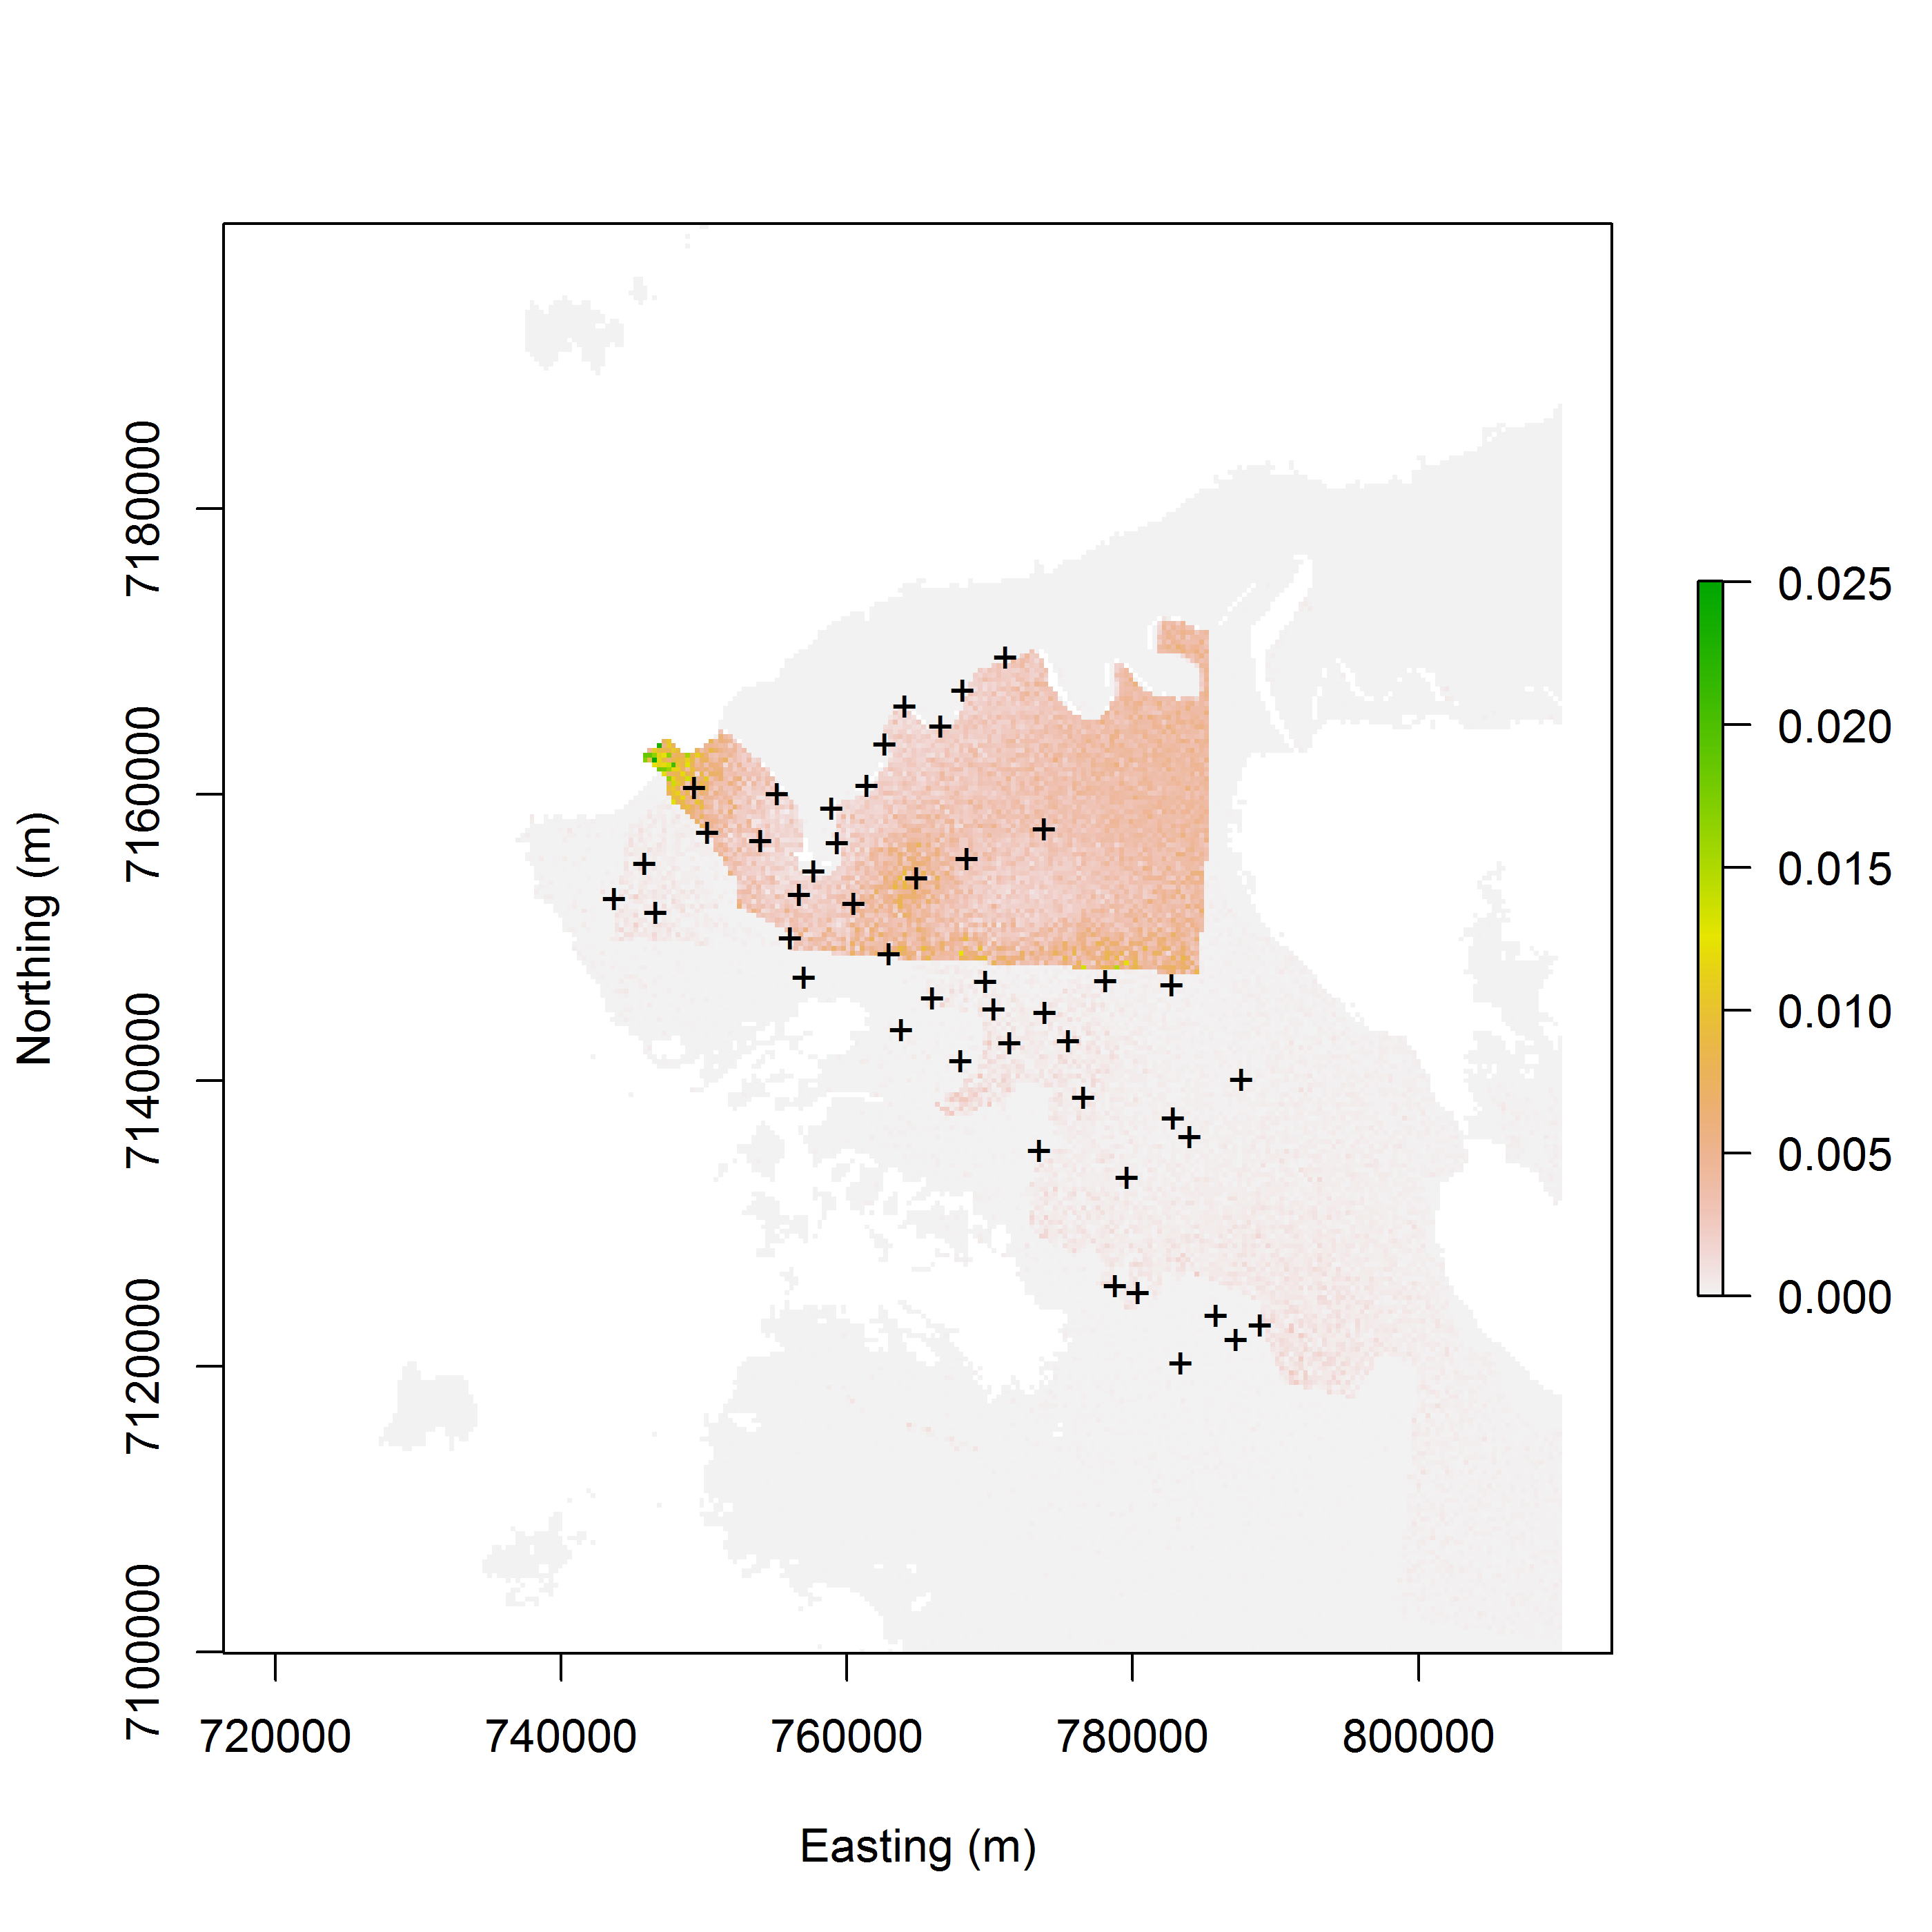
\includegraphics[width=3in,height=3in]{Ch11/figs/Dsurface34}
\label{ch9:fig:Dsurface}
\caption{Estimated density surface for the jaguar dataset}
\end{figure}


We note that there is room for improvement in our analysis. The
political boundaries used to demarcate protected areas are not as
concrete as we might like. In reality poaching pressure is likely to
be higher near remote park boundaries than in well-guarded park
interiors. One option
for addressing this would be to use a continuous measure of poaching
pressure such as distance from the nearest town, or some other
accessibility metric. It would also be interesting to model density
separately for each sex. Many of the detections outside of the park
were of males, and thus it is possible that the sexes use habitat
differently. Developing models for these two hypotheses could be
readily accomplished using slight modifications of the code found in
the \R~package \scrbook.



\section{Summary}

When state-space covariates are available,
density can be modeled by replacing the uniform prior on the activity
centers with a
prior based on a normalized log-linear function of covariates. This
distribution has been widely used in ecology to model point processes
as well as resource selection probability functions
\citep{manly_etal:2002,lele_keim:2006}. In the SCR
context, use of this new prior results in
a model for the inhomogeneous point process describing the
location of activity centers, which can be used to test hypotheses
about spatial variation in density. In
rare cases, these covariates are truly continuous in the sense that
they are defined as a function of space. More often, covariates are
represented as rasters, which simplifies the analysis. Fitting these
models can be accomplished using \bugs, \secr, or the custom \R~code
presented in this chapter and found in the package \scrbook.
%However,
%at the time this book was written, \scrbook is only software available
%for fitting models with covariates of both density and ecological
%distance.

All the examples in this section included a single state-space
covariate, but this was for simplicity only. Including multiple
covariates poses no additional challenges. Similarly, additional model
structure such sex-specific encounter rate parameters or behavioral
responses can be accommodated. Even more remarkable is the ability to
consider covariates that affect both density and ecological
distance. The ramifications of this are enormous for applied
ecological research and conservation efforts because, for instance,
researchers can use capture-recapture data to identify areas where
density is high, and to model important quantities such as landscape
connectivity \citep{royle_etal:2012ecol}. Addressing such questions
is simply not possible using standard, non-spatial capture-recapture
methods. Accomplishing these goals will of course require more data
than is needed to estimate the parameters of a basic SCR model.

